\documentclass[a4paper,leqno]{book}

\usepackage[T1]{fontenc}
\usepackage[utf8]{inputenc}
\usepackage[english]{babel}
%\usepackage{blindtext}
\usepackage{amsmath}

%\usepackage{array,tabularx,tabulary,booktabs}
\usepackage{longtable} 
\usepackage{multirow}
%\usepackage{wrapfig} 
\usepackage{graphicx}
\usepackage{algorithm2e}
\usepackage{listings}

%\hoffset=-5mm

\begin{document}
	


\date{2017/10/29}
\author{Bolshakova Liubov\\ Campagnoli Chiara\\ Lagni Luca}
\title{\textbf{\huge Travlendar+}\\ Requirement Analysis and Specification Document}
\frontmatter                            % only in book class (roman page #s)
\begin{minipage}[!t]{\linewidth}
	\centering
	
\includegraphics[scale=0.7]{logo2}
\end{minipage}
\begin{minipage}[!h]{\linewidth}
	\maketitle 
\end{minipage}
                             % Print title page.
\tableofcontents                        % Print table of contents
\mainmatter   

\chapter{Introduction}

\section{Purposes}
In this chapter we will decline all the goals that we have extract from our text and the actors that take part in the system and the environment of our application.

\subsection{Goals}

\begin{itemize}
\item (G01): The software should allow the user to register.
\item (G02): The system allows User to set his/her route inside a city or a region.
\item (G03): The system allows a User to choose a kind of transport among pre-defined travel means according to his/her preferences
\item (G04): The system allows a User to reserve a range of time for breaks.
\item (G05): The system must communicate to the user that a path (selected by this one) is not reachable or it's out of time.
\item (G06): The system must provide all the possible path that can be taken by a user, according to his/her needs.
\item (G07): The system must provide firstly the most optimized and suitable solution, according to the user preferences.
\item (G08): The system must provide information about problems/strikes for all the travel means  included in the software.
\item (G09): The system must provide a user the information about weather conditions during his/her planned route.
\item (G10): The system must provide a way to permit a user to buy a ticket for public transports.
\item (G11): The system must provide the nearest location of a bike provided by a pre-defined bike sharing service provider.
\item (G12): The system must provide the nearest location of a car provided by a pre-defined car sharing service provider.
\item (G13): The system must avoid overlaps in user's scheduled travels.
\item (G14): The system must allow the user to create meetings with different priority.
\item (G15): The system must inform the user about upcoming meetings.
\item (G16): The system must allow the user to change the part of the path during his/her trip.
\item (G17): The system must provide an alternative path in case of problems along the selected one.
\item (G18): The software should show a user, if possible, the combination of travel means that minimize the carbon footprint, according to the selected path and the required time.

\end{itemize}

\section{Scope}
\subsection{Description of the given problem}
Travlendar+ is a management service-to-be that allows users to plan their meetings and make  arranged routes to their destinations. The given problem is to design, implement and test a calendar-based application for it.
A user can create an appointment on a certain date, time and reachable location (over a region) using GPS localization. The appointment can be held either at a specific time or in a time interval and last for a certain time period. An appointment can be repeated regularly over time (lunch, gym, taking children to a kindergarten). A User can travel with someone else and can meet or leave them during the day.

User has an opportunity to use his own travel means and a pass for public transports. According to this the travel means can be grouped in three categories: public, shared or private.

\begin{itemize}
	\item Public transport: include trains, buses, underground, taxis, trains. They have to be taken in their designated stops. User must have a valid ticket in order to take any public transport but taxis (do not require tickets). Otherwise a User must have an availability to buy a ticket, update his/her pass or pay for a taxi trip on-line with his/her credit card;
	\item Shared travel means: include car and bike. They are located in specific places and require to make a reservation for using them;
	\item Private travel means: vehicles owned by the User. They can be cars, bikes, motorcycles. Walking is also a private travel means.
\end{itemize}

Weather conditions can change during the day. A User can find out the actual information about the latest weather conditions during his/her planned meeting and choose more comfortable way to reach his/her final destination.

In the morning or on demand a User can send a request about the schedule of his/her daily appointments by some criteria of evaluation such as assigned priority and satisfaction of constraints imposed by the User. When a new appointment is made, a User creates a new item in the application and saves it in the appointment list. User can require the application rescheduling meetings because of unexpected changes (e.g. cancelled or postponed meeting). User always know how long it takes to get his/her final destination. 

A green and ecological approach is the core of Travlendar+ business and according to this a lot of details have been defined:  the application firstly suggests the most ecological path to a User (e.g. path with walking or using public transport means, a bike instead of a car) to minimize carbon footprint. 
Ultimately, the system will have to be easy-to-use, reliable and highly scalable to fit perfectly  with the mutable context in which it will be planned to be used.


\subsection{World phenomena}

\begin{itemize}
	\item User arranges a new meeting;
	\item User meets another person;
	\item User leaves another person:
	\item User has private travel means and/or passes for public transportation;
	\item User gets up;
	\item User moves;
	\item Shared travel mean moves;
	\item User's pass expires; 
	\item There are available various travel means.
\end{itemize}

\subsection{Shared phenomena}

\begin{itemize}
	\item Allocation of a  shared transport;
	\item User's allocation;
	\item Shared travel mean is not available;
	\item Weather condition changes;
	\item Public transport reaches its final stop;
	\item Public transports are not available due to a strike or an accident;
	\item User requires a timetable of the necessary public transport route;
	\item User inserts a new appointment into the calendar;
	\item User buys a ticket or a pass for the necessary public transport;
	\item User requires booking his/her ride.	 
\end{itemize}

\subsection{Machine phenomena}
\begin{itemize}
	\item meetings scheduling;
	\item creating a new instance of Travlendar's classes;
	\item database queries about Client;
	\item storing routes' history;
	\item computation the fastest path;
	\item building the most ecological path;
	\item transfering a User to external services with API;
	\item generating a warning about unreachable time;
	\item generating a notification about upcoming meeting.
\end{itemize}

\section{Definitions,acronyms and abbreviations}
\subsection{Definitions}
\begin{itemize}
	\item Appointment: a business meeting with high priority.
	\item Client: a registered user.
	\item Dangerous path: a path which requires crossing districts or areas with potential risk, such as high criminality.
	\item External company: a general external company that provides travel means or services.
	\item Meeting: an event which is created by a User for satisfying his/her needs.
	\item Owning company: a stakeholder
	\item Path: a trajectory between initial and final point of the route.
	\item Private travel means: vehicles owned by the User. They can be cars, bikes, motorcycles. Walking is also a private travel means.
	\item Public transport: include trains, buses, underground, taxis, trains. They have to be taken in their designated stops. User must have a valid ticket in order to take any public transport but taxis (do not require tickets). Otherwise a User must have an availability to buy a ticket, update his/her pass or pay for a taxi trip on-line with his/her credit card.
	\item RESTful way:  representational state transfer, a way of providing interoperability between computer systems on the Internet.
	\item Route: a way how to reach the destination of the meeting.
	\item Shared travel means: include car and bike. They are located in specific places and require to make a reservation for using them.
	\item Technical Support: an actor who aids the user in case of techical problems with the app.
	\item Trip: a piece of a route in which only one travel mean is used.
	\item User: a general actor who uses the application.
	\item Visitor: a user who is not registered yet.
\end{itemize}

\subsection{Acronyms}
\begin{itemize}
	\item API: Application Programming Interface.
	\item GPS: Global Positioning System.
	\item GSM: Global System for Mobile Communications.
	\item GUI: Graphical User Interface.
	\item OAMOT: Other Autonomous Means of Transport
	\item ONAMOT: Other Non-Autonomous Means of Transport
	\item OS: Operating System.
	\item RAM: Random-access memory.
	\item RASD: Requirement analysis and Specification Document.
	\item SMS: Short Message Service.
\end{itemize}


\subsection{Abbreviations}
\begin{itemize}
	\item (An): n-actor.
	\item (ARn): n-availability requirement.
	\item [DAn]: n-domain assumption.
	\item (Gn): n-goal.
	\item (HIn): n-hardware interface.
	\item (HLn): n-hardware limitation.
	\item (MRn): n-maintainability requirement.
	\item (MIn): n-communication interface.
	\item (Mn): n-predefined travel mean.
	\item (OCn):n-other constraint.
	\item (PRn):n-performance requirement.
	\item (PtRn): n-portability requirement.
	\item (REn): n-functional requirement.
	\item (RRn): n-reliability requirement.
	\item (Sn): n-stakeholder.
	\item (Scn): n-scenario.
	\item (SCn): n-standard compliance.
	\item (SIn): n-software interface.
	\item (SRn): n-security requirement.
	\item (UIn): n-user interface.
	\item (UC.n): n-use case.
	
\end{itemize}



\section{Document Structure}

Besides introduction, this RASD is composed of 4 parts:

\begin{enumerate}
	\item Overall description: in this chapter we include further details about product functionalities, user characteristics, domain assumptions and constraints. In particular, we identify actors and stakeholders and involved means of transport, class diagrams and statecharts.
	\item Specific requirements: in this chapter we include an overview about interfaces that will be needed, a set of possible scenarios and derived use cases, use cases diagrams and sequence and activity diagrams, more specific design constraints and non functional software attributes.
	\item  Formal analysis using alloy: in this chapter we include our alloy model with the obtained results.
	\item  Effort spent: in this chapter we include the amount of hours spent on the work by each group member.
\end{enumerate}

\section{Reference Documents}
\begin{itemize}
	\item Mandatory Project Assignments.pdf
	\item RASD sample from A.Y. 2016-2017
	\item http://alloy.mit.edu/alloy/tutorials (for deep documentation about alloy)
	\item http://ieeexplore.ieee.org/document/720574/?reload=true (830-1998 - IEEE Recommended Practice for Software Requirements Specifications)
	\item moovitapp.com (for analysing similar applications)
	\item Amedeo E.,UML Pocket, APOGEO s.r.l., 2007 (for deeper understanding UML diagrams making) 
\end{itemize}



\chapter{OVERALL DESCRIPTION}

\newpage
\section{Product Perspective}

\subsection{Class diagram}
\begin{figure}[!h]
	\begin{center}
		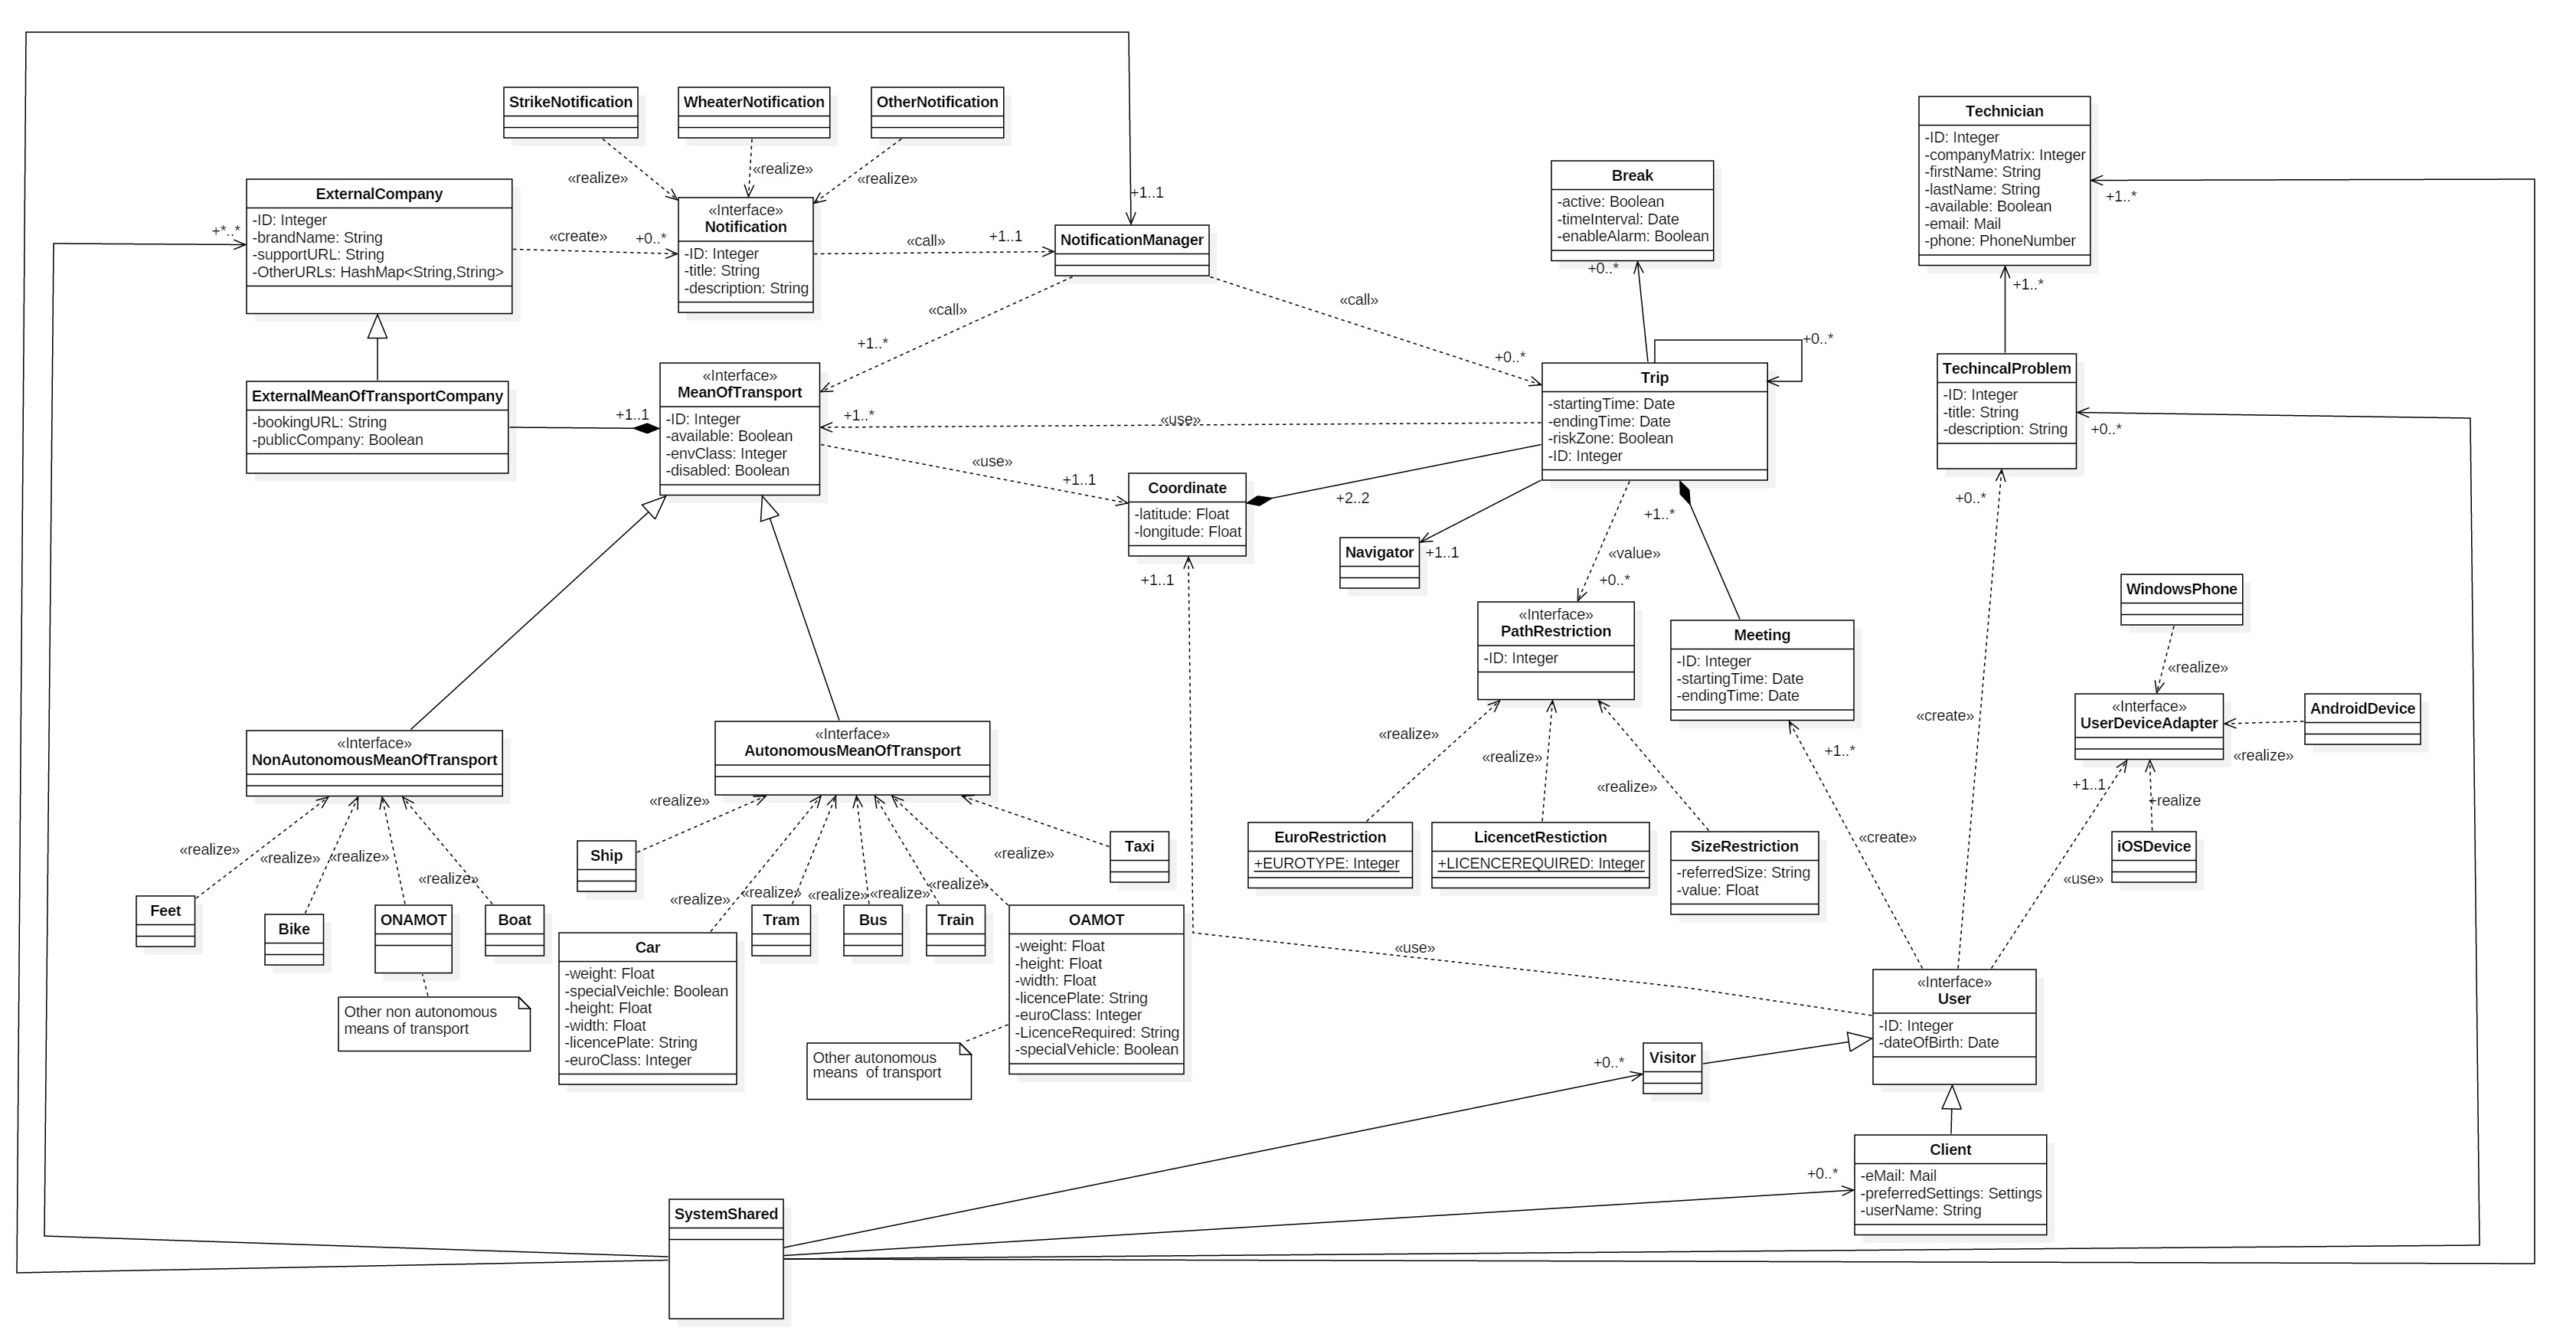
\includegraphics[scale=0.15, angle=90]{TravalendarPlusClassDiagramFull_29102017_1}
	\end{center}
	\caption{Class diagram}
\end{figure}

\newpage
\subsection{Statecharts}
\begin{figure}[!h]
	\begin{centering}
		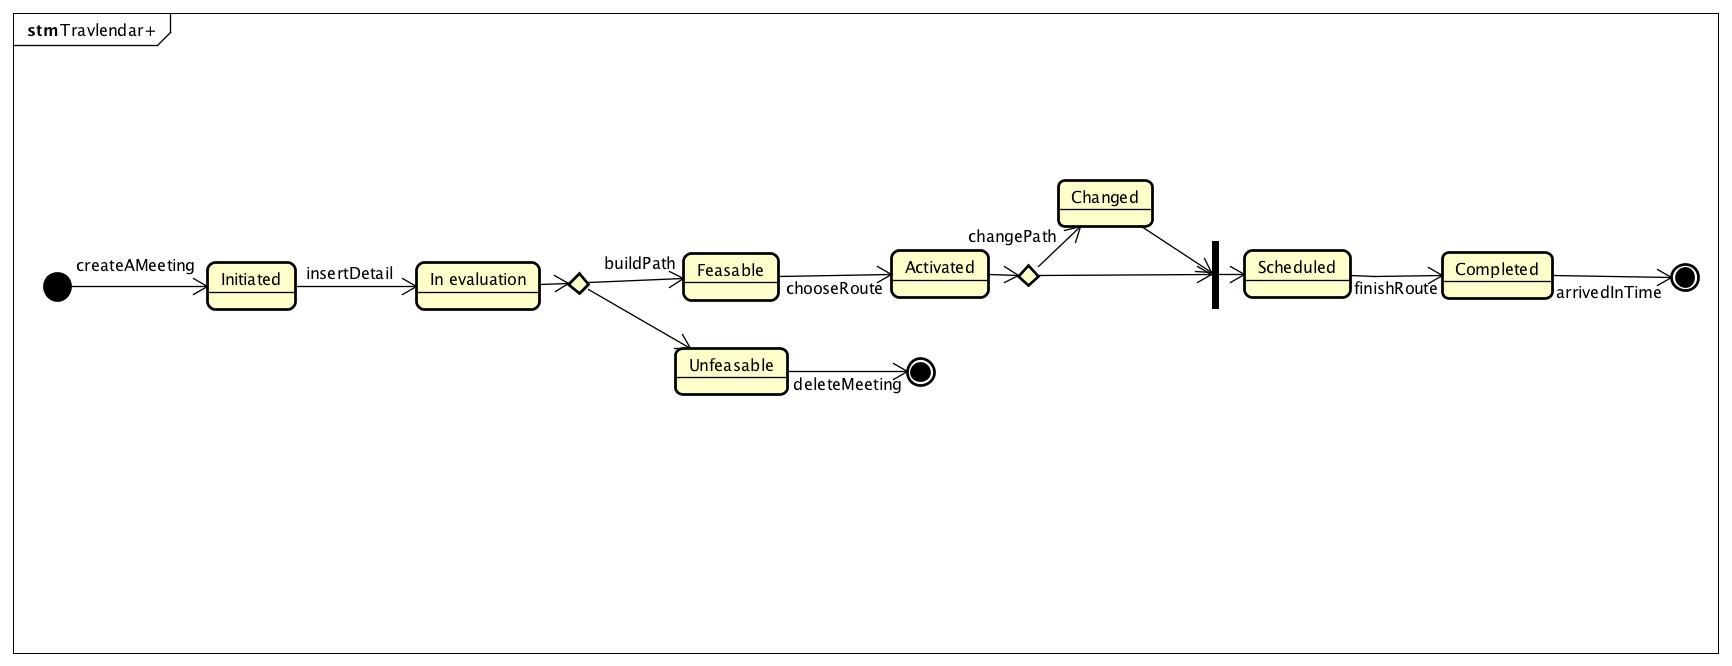
\includegraphics[scale=0.3, angle=90]{StatechartDiagram_28102017_2}
		\end{centering}
	\caption{Meeting statechart}
\end{figure}

\newpage
\section{Product Functions}
Here we include the most important requirements of our software

\begin{itemize}
	
	\item (RE01): The system must allow users to sign in.
	\item (RE02): The system must allow the client to log in.
	\item (RE03): The system must allow the client to log out.
	\item (RE04): The system must allow the client to delete his account.
	\item (RE05): The system must provide a high level of security for client's data.
	\item (RE06): The software must have an access to all major mobile devices whose OS is Android OS, iOS and Windows Phone.
	\item (RE07): The software must interface with all major public transport companies that provide API.
	\item (RE08): The software must allow the user to choose a route.
	\item (RE09): The software must allow the user to define time constraint to a specific selected route.
	\item (RE10): For each path the software must provide all the available means of transport that can be used, according to the software interfaces.
	\item (RE11): The software must allow the user to select vehicles that he/she wants to use for the route.
	\item (RE12): The software must require the estimated time for a break.
	\item (RE13): If a route is not possible because of overlaps with other journeys, the application must deny that option and notify the user.
	\item (RE14): If a route is not possible because the required time to reach the destination is not enough, the application must deny that option and notify the user.
	\item (RE15): If a route is not possible because the selected travel mean is not allowed to pass a specific place, the application must deny that option and notify the user.
	\item (RE16): If a route is not possible because breaks requires too much time, the application must deny that option and notify the user.
	\item (RE17): The software must provide a User all the available solutions, according to his/her selected preferences, to get from one place to another.
	\item (RE18): The software must inform the user about problems with using some transport (strikes , road damages, rain and so on) for which the usability is not guaranteed.
	\item (RE19): The application should provide, as first option, the optimal solution according to the users's preferences about minimizing carbon footprint.
	\item (RE20): If a break runs out the selected time the application must notify the user.
	\item (RE21): The application should avoid to make the user pass through dangerous zones of a city or a region.
	\item (RE22): If the user has to pass through a dangeousr zone, the application must inform him/her.
	\item (RE23):  The software must require the estimated time for a meeting.
	\item (RE24): For each meeting, the system should ask the user to define its priority (1-business, 2-appointment, 3-with friends, 4-personal).
	\item (RE25): The system should warn about upcoming meetings twenty minutes before.
\end{itemize}

\section{User Characteristics}
\subsection{Actors}
\begin{itemize}
	\item (A01): User - a general actor who uses the application.
		\item (A02): Client - a registered user.
		\item (A03): Visitor - a user who is not registered yet.
	\item (A04): Technical Support - an actor who aids the user in case of techical problems with the app.
	\item (A05): [External companies]
\end{itemize}

We have done a distinction between Client and Visitor because we think that , one day, 
it will be usefull , for our application, to evolved and a special treatment for making the 
user fidelity stronger will be desiderable or required.

Anyway, at this stage , there are no difference in features between a visitor and a client. 
So, if it is not necessary, we will refer to them as users.

\subsection{Agents}

The purpose of this application is to aim clients for short travels, so we limits our travel means:

\begin{itemize}

\item (M01): Feet 
\item (M02): Personal bike 
\item (M03): Personal car
\item (M04): Other autonomous personal means of transport
\item (M05): Other non autonomous personal means of transport
\item (M06): Bike provided by a bike sharing provider, if available
\item (M07): Car provided by a car sharing provider, if available
\item (M08): Other non autonomous transport
\item (M09): Other autonomous transport
\item (M10): Train
\item (M11): Tram
\item (M12): Bus 
\item (M13): Taxi
\item (M14): Metro (for Milan, Rome, Turin and Naples)
\item (M15): Boat (for cities like Venice).

\end{itemize}

We can exclude planes, because of the nature of the travels considered.\\

Other autonomous personal means of transport can be anything that has an engine like motorcycles , quad, segway and so on.

Other non autonomous personal means of transport can be anything, used for moving from one place to another, that hasn't an engine like rollerblade, skateboards and so on.

Other non autonomous means of transport can be tandems. 

Other autonomous means of transport can be rented vehicles like motorcycles , cars not provided by a carsharing but also hichkicking and so on.

For all the "other [...] transport" we don't provide a specialized definition, we only focus on maximum speed, euro class and possible special access/limitations (like for vehicles disposed for disable people). We assume mandatory (the client must provided this kind of information if he intended to use this kind of vehicles), if the user want to use this application correctly, and we leave the possibility to add information about other important things of that travel mean by the user himself.


\subsection{Stakeholders}
\begin{itemize}

\item (S01): Owning company - obviously, this company is a stakeholder.
\item (S02): External company - A general external company that provides means of transport or services. (Google, ATM, Mobike).

\end{itemize}

We can assume that another possible stakeholder could be the city (or region) government itself because the local community can be interested in investing resources for reducing traffic and pollution.\\

\section{Assumptions, Dependencies and Constraints}

\subsection{Domain assumptions}
Here we state the assumptions we made about the world interacting with the system:\\

[DA01] The user will drive only if in possess of a valid driving licence and respecting the law of the country and the area.
\newline
[DA02] Users subscribed to a car-sharing service know and respect the rules of such service.
\newline
[DA03] Only users subscribed to a vehicle-sharing service are able to drive vehicles of such service.
\newline
[DA04] The user will use public transport only if in possess of a valid ticket or travel pass and is aware of sanctions applied by public transport companies.
\newline
[DA05] The information inserted by the user on his profile is reliable and updated.
\newline
[DA06] Users will not try to login using another user's credentials.
\newline
[DA07] Every user can register to the system only once.
\newline
[DA08] The position of the user is always available whithin using our system.
\newline
[DA09] The information about the position of the user provided by the GPS is reliable.
\newline
[DA10] The interacting companies, such as public transport companies, vehicle-sharing services, weather forecast services, agree on cooperating and offering the system the services it needs to work.
\newline
[DA11] The information provided by companies of public transport (time-tables, ticket prices and anything related to possible problems of mobility, such as strikes, accidents or variations of path) are reliable.
\newline
[DA12] The information provided by companies of vehicle-sharing services (location of vehicles, prices) are reliable.
\newline
[DA13] The information provided by weather forecast services are reliable.
\newline[DA14] The public transport companies provide a service for purchasing tickets online.

\subsection{Constraints}
The system will only store data about registered users, after asking for their permission during the registration process. This data won't be used for any commercial purposes but only for the app's purposes and as stated in the terms of agreement.

\newpage
\subsection{Proposed system}
We will implement a system based on a client-server architecture and the common REST APIs to manage mobile application. A database server is needed to store the data of clients and extra-links for connecting with external companies in case of some problems with APIs. A possible framework for the application server is Spring, a java based framework. To connect with external companies the system will use HTTP protocol and proxy server is needed to receive requests from them and users.

\begin{figure}[!h]
	\begin{centering}
		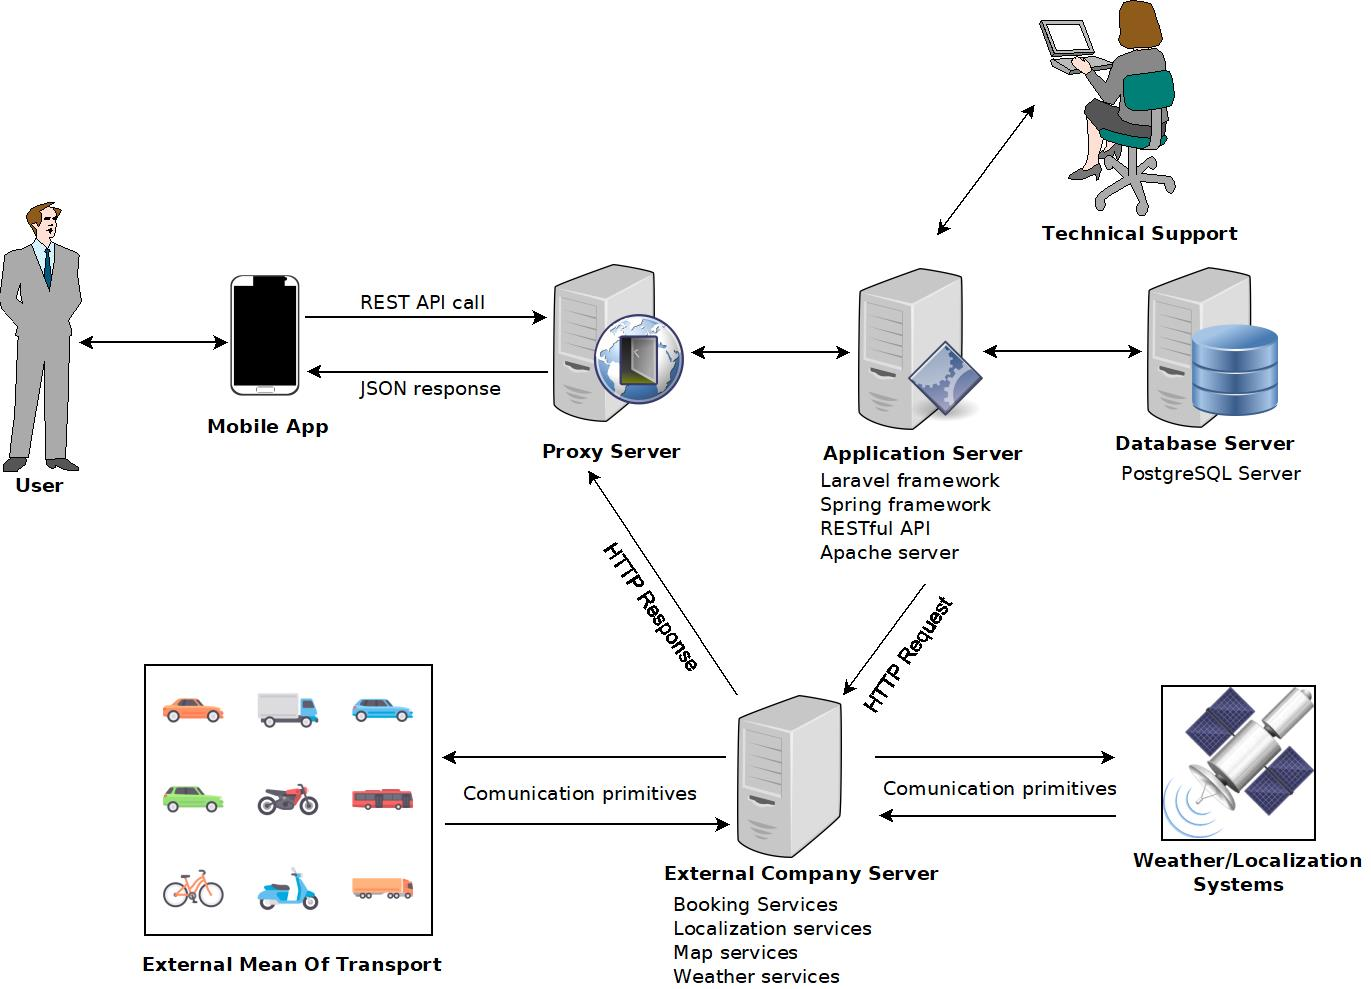
\includegraphics[scale=0.3]{ProposedSystemDiagram_29102017_1}
	\end{centering}
	\caption{Meeting statechart}
\end{figure}


\chapter{SPECIFIC REQUIREMENTS}

\section{External Interface Requirements}

\subsection{User Interfaces}
The section above shows the main interfaces between the user and the app 
\begin{itemize}
\item (UI01): The user has to interface with the route planner of the app
\item (UI02): The user has to interface with the navigator of the app.
\item (UI03): The user has to be allowed to interface with the technical support.
\item (UI04): The user has to be allowed to interface with the means of transport according to the selection of the app.
\item (UI05): The user has to be allowed to interface with external companies for booking methods via the app.
\end{itemize}

Moreover , the application must provide support for disable users like:
\begin{itemize}

\item (UI07):Support for users that have low level limitations and, because of this condition, cannot access the application in the standard way (like people with low vision disease). 
\item (UI08):Support for users that have high level limitation and , because of that, cannot use specific means of transport (like old people or people with movements limitation).

\end{itemize}

\subsection{Software Interface}
This section shows the main interfaces between the application and the software provided by the user/client's device.

\begin{itemize}
\item (SI01): The application must interface with the localization device disposed by the client/user's device.
\item (SI02): The application must interface with the system notification of the client/user's device.
\item (SI03): The application must interface with the standard I/O ways of interaction of the client/user's device.
\item (SI04): The application should interface with the system clock widget of the client's device.
\item (SI05): The application should interface with the language selection of the system.
\item (SI06): The application must provide, in addition to the standard GUI, a low and high contrast mode. 
\item (SI08): The application must interface with external companies API (those who are contemplated), in order to provide a way to access to transport's data.
\end{itemize}

\subsection{Hardware Interfaces}
This section shows the main interfaces between the software or client/user or application and the hardware of the client/user's device

\begin{itemize}
\item (HI01): The client's device must access to the Internet.
\item (HI02): The client's device must manage geolocalization. 
\end{itemize}

\subsection{Communication Interfaces}

\begin{itemize}
\item (MI01): The system must have a TCP/IP protocol.
\item (MI02): The system must have a way to manage the GSM protocol.
\item (MI03): The user device must have a way to manage 3G or wi-fi protocols.
\item (MI04): The user's device must have an I/O interface (like touch screen).
\item (MI05): The communication between the application and the user must have a RESTful way .
\end{itemize}

\section{Functional Requirements}

\subsection{Scenarios}
In this section we provide some possible situations that can occours during the use of our application.

\subsubsection{Scenario (Sc01) }
Albert has an important appointment in Milan. 
This meeting could provide a new customer to his company, so he has to do a good impession, arriving in time.\\
He arrived by train at 8.00 in the morning and the meeting is scheduled for 11.15, there is a lot of time, because 
the company is near the station, but he doesn't know where to go.\\
He is already a client of our app, because he travels a lot for work.\\
He sets up the initial point (using his current position) and the arrival point.\\
The path is very short, and there are no car/bike sharing near with him (the application doesn't provide them), but he doesn't go by foot not to sweat,
so he disable foot option and decide to use the bus, which come closer to his arrival.\\
The application provides a link connection to the ATM site for reserving a ticket, and he uses it.
The total time of the travel is 30 minutes so he has to decide what to do during this time interval.
He has seen that there is a library near the company, it's only 5 minutes by foot, so he decides to set a break here that longs 3h, for review his presentation,
but this break requires too much time and, because of this, the software doesn't allow him, so he has to change it in only 2h.
There are no problems during the path and arrived at the library at 8.40.\\
At 10.40 the alarm related to the break rings, so he decides to leave the library and go to the company building. 
Here he disables the app.

\subsubsection{Scenario (Sc02) }
Brigitte is a french tourist who decided to visit Venice. She's at the airport right now and she wants to go to her hotel .\\
This is her first time in Italy so she looks in the play store and find out our app.
She doesn't travel very often , so she decides to use the app as a visitor.\\
First of all, she decides just to get the hotel to leave her luggage.
She sets the application, she only chooses public and shared means of transport. 
She decides to use the bus (for the first part of the journey) to reach the hotel and  it takes only 5 minutes by foot. 
She doesn't set any breaks and it requires a path time of 1h.\\
After she has arrived to the hotel, she decided to visit Piazza San Marco, Palazzo Ducale and Ponte di Rialto in her first day.
She has all the day, but she has to come back to the hotel before 2 A.M.\\
Her first place is Piazza San Marco, which is not so distant from her hotel , so she sets the walking option. 
After she has been here, she sets Palazzo Ducale as the next place and a break of 1.30h for enjoying Piazza San Marco.\\
For Palazzo Ducale there are only four means of transport suitable: walking, car sharing, bike sharing and taxis, because it is a bus strike at that moment. 
She decides to take a taxi,but she doesn't call it because she has enough time,  she wants to relax and takes it easy , she's on holiday after all.\\
After 1.30h the alarm rings, but she has changed her mind  and decided to go there by the bike sharing (because she take a Cappuccino and a Croissan at piazza San Marco and she had to paid 20 euro, that's why she has decided to save money). 
Our application provides her an external link to the Mobike application that shows her the nearest available bike and the way how to unlock it.
She does and goes to Palazzo Ducale.\\
She arrived at 4.00 and decides to set a journey to ponte di Rialto via Gondola (using a boat) , the last available will be at 5.15, so she sets the required time to arrive here on bike and a 30 minute break.\\
But her break requires too much time, and she ignores the application notification.
So, now, she has to arrive there in only 10 minutes , the only possible solution is the taxi and she has to do so.\\
Our application doesn't has a direct access to the API of the taxi provider because there has not been released yet but she can call a taxi using our link to the taxi site and then, using the contact provided, call for a taxi reservation. She does so.\\
She buys the ticket for the boat directly there. 
The tour finishes at 18.30.\\
Then she decides to go to a Disco and sets the arrival time at 23.00.
Only taxis, bike sharing and car sharing are available, but as she wants to use a car (she has to pass through a risk zone) she decides to rent a car.\\
After the Disco she decides to eat someting and visit some shops there. 
She delays her departure and the application informs her that there are no available solutions for arriving in time. She only exits from the app.\\
Then , at 1.30 she sets the path to come back to the hotel without any breaks and selects the car as a mean of tranport. Once she arrives at the hotel , she disables the app.\\

\subsubsection{Scenario (Sc03) }
Carl has to marry , her future wife (Denise) has decided the place where to do so.\\
She is from Mantova and he is from Sicily (like all his parents and friends).\\
Denise lived in Mantova since she was 23 and then she decided to move to Sicily where she met Carl, her family is in Mantova and, sometimes she goes to find them (and of course knows the city) but Carl has never been there.
So, Carl is in big troubles because he only has 30 minutes to reach Santuario della Beata vergine delle Grazie from the Mantova train station and, of course, he has to find a way to carry also all his family and friends (which are , at last 30).
So he is in a hurry and decides to download the app and use it as a visitor.\\
He sets the journey without breaks and there are no public possible solutions that can be adapted, and there is only one possible proprietary solution that provide API : to call a taxi.\\
This is a problem because for carrying all his parents and friends it will require at least 5 taxis.\\
But there is another option, provided by an external company , which rent bus.\\
The company doesn't provide any api, but it provides a link for their site in which there are all their contacts.\\
This is the way he used our app, we don't know if he can accomplish his mission , we can suppose so by the fact that he doesn't used the app anymore for that day.\\
We pray for you Carl!\\

\subsubsection{Scenario (Sc04)}
Peter is a user of Travlendar+ app. He and his family with two children arranged with their friends about the trip to Gardaland park in advance and decided to put it in the app’s calendar. One of the most convenient way to travel with children is using a car, that’s why one of Peter’s user preferences is a car option. It is Sunday, there is no traffic jams anywhere. So the app suggests a car option as one of the travel means to reach the location of the meeting. Peter, surely, chooses this option. It is the first time of using this option and then the app asks him if he has his own car. Peter does and accepts this option. The app asks to allow to remember his decision for the next trips and whishes him a nice day!

\subsubsection{Scenario (Sc05)}
Chiara has just got to hear about a very interesting exhibition in Palazzo Reale dedicated to her favorite painter Toulouse-Lautrec and she is looking forward to visiting it. She decides not to postpone the visit and wants to go there instantly. She opens Travlendar+ app and creates an appointment. Unfortunately, she is in Biccoca, it is 18:55 now but Palazzo Reale closes at 7 pm.   The app warns Chiara that she cannot get to the exhibition because of unreachable time. Chiara postpones the visiting for tomorrow.

\subsubsection{Scenario (Sc06)}
Diana would like to go to the city center to walk with her boyfriend. Diana has already used Travlendar+ and creates the appointment. The application suggests her different ways to reach her destination. Diana loves bicycling and she has enough time before the date. She chooses the bike way. The application asks her if she has her own bike. Unfortunately, Diana has just moved into Milan and has not had her own bike yet. She answers “No” and the app suggests her the bike-sharing option. It is exactly what she needs and she chooses it. 

However, the bike-sharing service site with API does not work now. The app notifies the Technical support about the problem. The application shows a message with apologising to Diana and asking her a few minute waiting. The Technical support fixes the problem with redirecting to the page with a link to another bike-sharing service without open API.  As soon as the problem is fixed Diana gets a notification that she is able to reserve a bike with this link. Diana is happy, but her wishing to have her own bike has increased.

\subsubsection{Scenario (Sc07)}
Paolo is a student living in Milan. He is already registered to the app and has a bike on his own, which is saved in the personal settings of his account.\\
He has an exam this afternoon and he creates it as a meeting with high priority. As Paolo is really concerned with environmental issues, he sets the "Minimize carbon footprint" option.\\
The best choice, according to his preferances and the distance of the university, would be the bike; however it is a very rainy day and the system excludes this possibility, due to the bad weather conditions.
The proposed route is therefore the bus. Paolo selects this route and reaches his university in time to study a little bit before the exam.

\newpage
\subsection{Use cases}
\subsubsection{Use case diagram}
\begin{figure}[!h]
	\begin{center}
		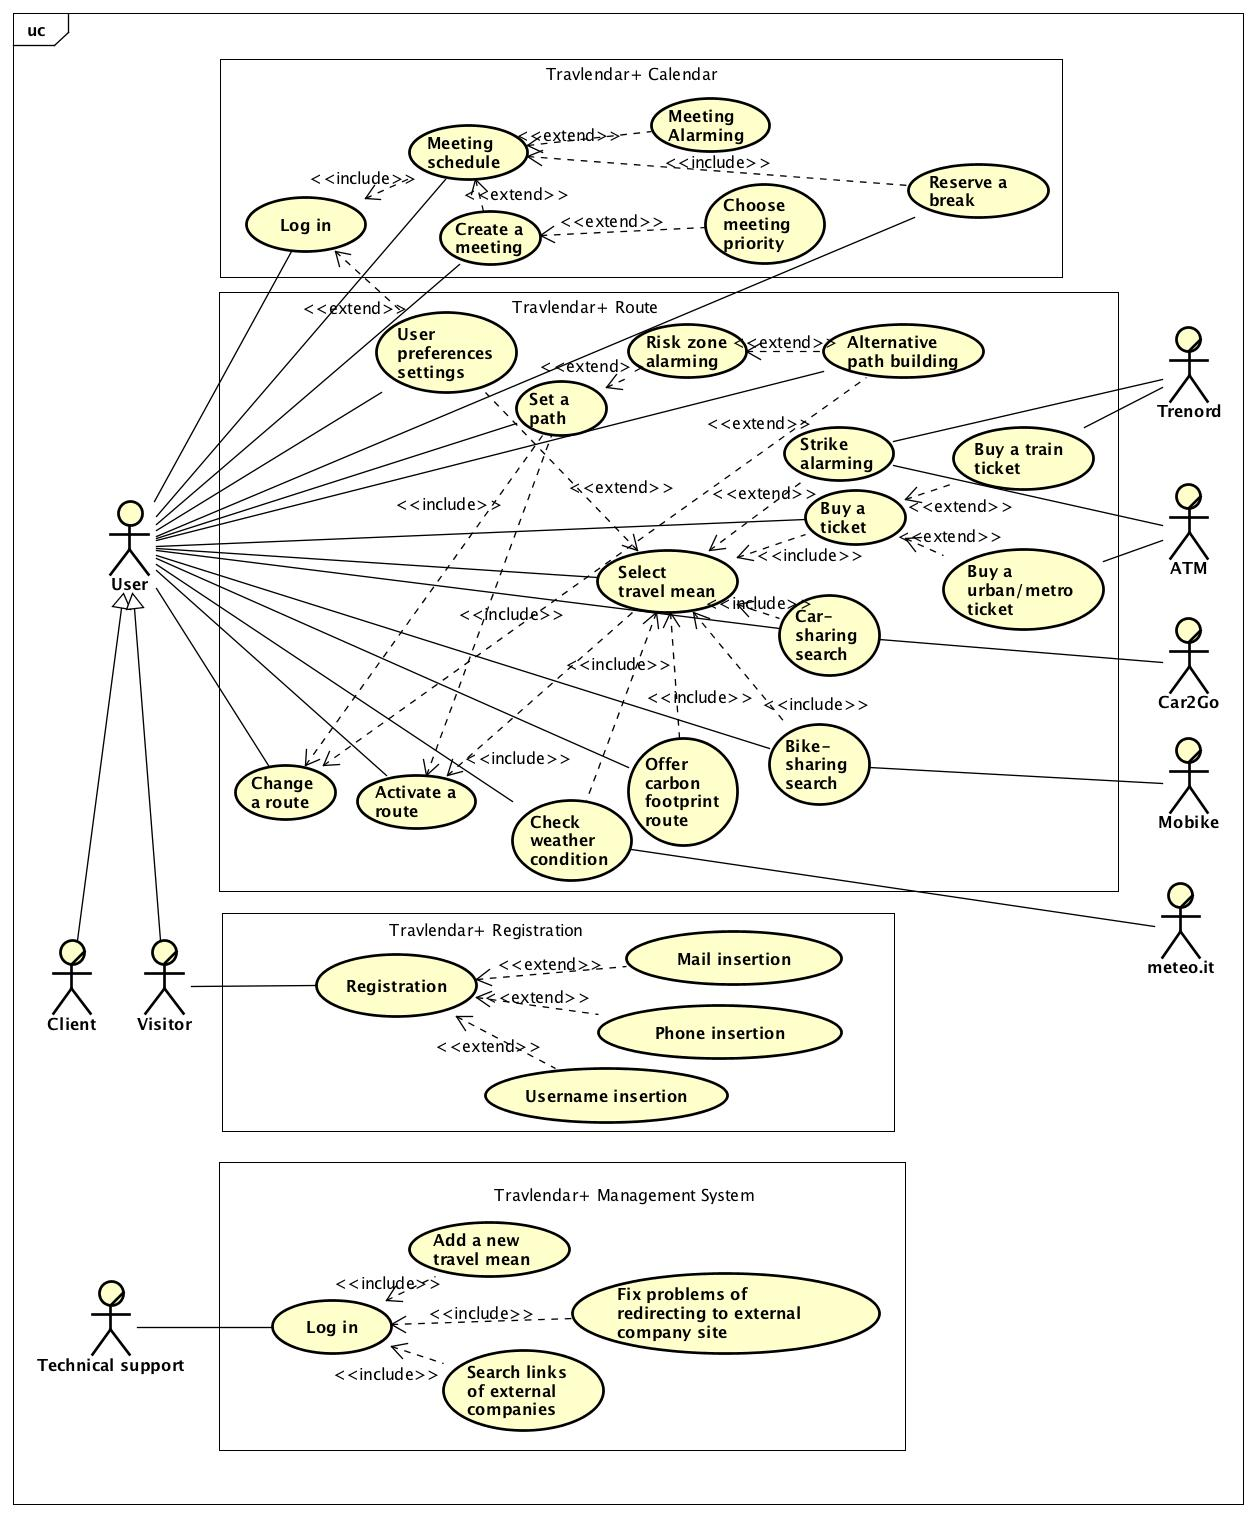
\includegraphics[scale=0.3]{UseCaseDiagram_28102017_1}
	\end{center}
\end{figure}
\newpage

\subsubsection{Use case 1. Visitor registers in the Travlendar+ system}

\begin{table}[!h]
	\centering
	\begin{tabular}{|l|l|}
		\hline
		\textbf{Actors}         & Visitor  \\ \hline
		\textbf{Goals }            & {[}G01{]}  \\ \hline
		\textbf{Input conditions}  & \begin{tabular}[c]{@{}l@{}}1. The Visitor has an Internet access.\\ 2. The Visitor is on the home page.\end{tabular}  \\ \hline
		\textbf{Events flow}     & \begin{tabular}[c]{@{}l@{}}1. The Visitor clicks on the “Sign in” button on the home page to start \\ the registration process. \\ 2. The Visitor fills all mandatory fields.\\ 3. The Visitor clicks on the “Confirm” button.\\ 4. The system saves the data.\\ 5. The system sends a SMS to the new User with the password.\end{tabular} \\ \hline
		\textbf{Output conditions} & \begin{tabular}[c]{@{}l@{}}The Visitor ends the registration process successfully and become a new \\ User. From now on he/she can log in to the application \\ providing his/her credentials.\end{tabular}  \\ \hline
		\textbf{Exceptions}        & \begin{tabular}[c]{@{}l@{}}1. The Visitor is already registered.\\ 2. The Visitor inputs incorrect data in one or more mandatory fields.\\ 3. The Visitor takes a username that has already been associated with \\ another User.\\ 4. The Visitor chooses an email that has already been in the system.\\ \\ All exceptions are handled with notifying the issue to the Visitor and \\ taking back to the point 2 of Events Flow.\end{tabular} \\ \hline
	\end{tabular}
\end{table}


\subsubsection{Use case 2.User logs in}

\begin{table}[!h]
	\centering
	\begin{tabular}{|l|l|}
		\hline
		Actors            & User  \\ \hline
		Goals             & {[}G01{]}  \\ \hline
		Input conditions  & The User is on the home page.   \\ \hline
		Events flow       & \begin{tabular}[c]{@{}l@{}}1. The User inputs his/her credentials into the “Username” and \\“Password” fields.\\ 2. The User clicks on the “Log in” button to get access.\\ 3. The system redirects the User to his/her personal area.\end{tabular}  \\ \hline
		Output conditions & The User gets access to his/her personal area successfully.  \\ \hline
		Exceptions        & \begin{tabular}[c]{@{}l@{}}1. The User inputs invalid Username.\\ 2. The User inputs invalid Password.\\ All exceptions are handled with notifying the issue to the User and \\taking back to the point 2 of Events Flow.\\ \\ 3. The User inputs invalid Password 5 times.\\ The exception is handled with notifying the issue the User and \\offering to change his/her password.\end{tabular} \\ \hline
	\end{tabular}
\end{table}

\newpage
\subsubsection{Use case 3.User sets the path to the necessary location}

\begin{table}[!h]
	\centering
	\begin{tabular}{|l|l|}
		\hline
		Actors            & User  \\ \hline
		Goals             & {[}G02{]} \\ \hline
		Input conditions  & \begin{tabular}[c]{@{}l@{}}The User is on the home page.\\ GPS navigator is on.\end{tabular}    \\ \hline
		Events flow       & \begin{tabular}[c]{@{}l@{}}1. The User selects the option “Set the route”. \\ 2. User sets up the initial point using GPS localization.\\ 3. The User sets up the arrival point using GPS localization or specified address.\\ 4. The User checks if his/her current position and the arrival point has been\\ correctly defined.\\ 5. The User clicks on the “Confirm” button.\\ 6. The system builds the route. \\ 7. The system offers the User the ways in order of increasing their length.\end{tabular} \\ \hline
		Output conditions & The User gets the set of routes to reach his/her destination.  \\ \hline
		Exceptions        & \begin{tabular}[c]{@{}l@{}}1. GPS is out of work.\\ 2. The User inputs the coordinates of initial and arrival point indifferent regions.\\ 3. The User’s current position cannot be defined correctly.\\ 4. It’s impossible to build the route inside the city/region.\\ \\ All exceptions are handled with notifying the issue to the User and taking back \\to the point 2 of Events Flow.\end{tabular}  \\ \hline
	\end{tabular}
\end{table}

\begin{figure}[!h]
	\begin{center}
		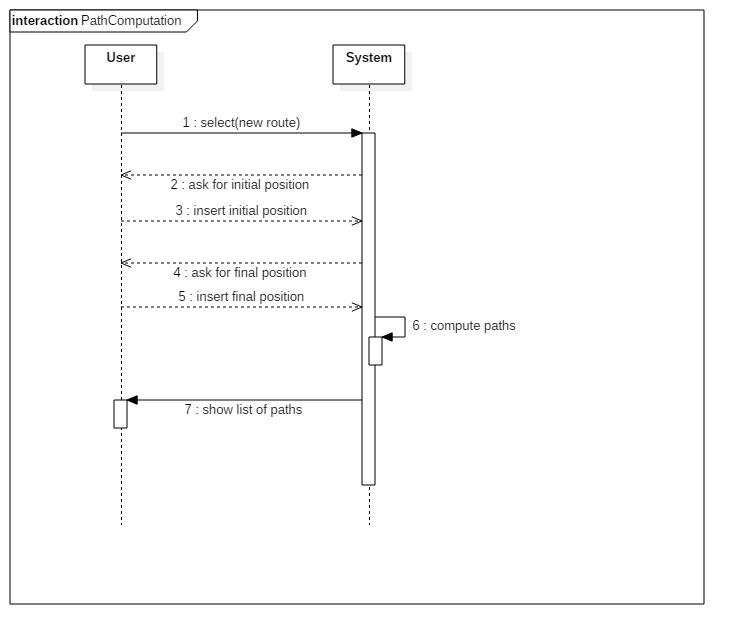
\includegraphics[scale=0.3]{PathComputation_seq_271017_1}
	\end{center}
	\caption{Path setting sequence diagram}
\end{figure}

\newpage
\begin{figure}[!h]
	\begin{center}
		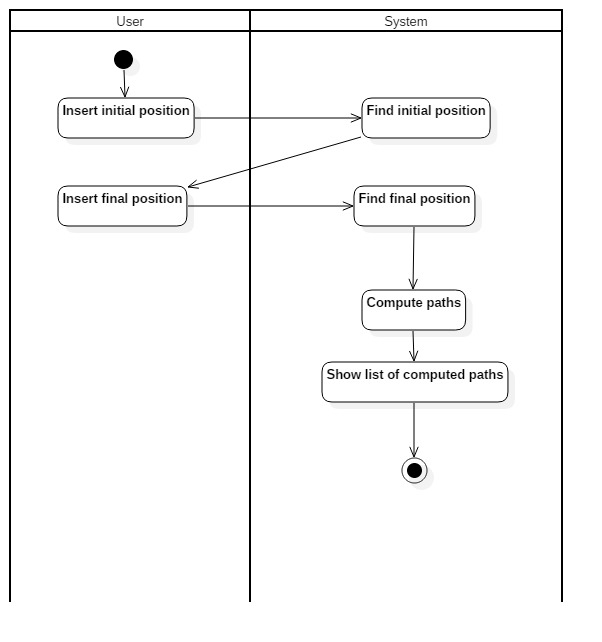
\includegraphics[scale=0.3]{PathComputation_act_271017_1}
	\end{center}
	\caption{Path setting activity diagram}
\end{figure}


\subsubsection{Use case 4 .User defines his/her preferable travel means}

\begin{table}[!h]
	\begin{tabular}{|l|l|}
		\hline
		Actors            & User\\ \hline
		Goals             & {[}G03{]} \\ \hline
		Input conditions  & The User has logged in.  \\ \hline
		Events flow       & \begin{tabular}[c]{@{}l@{}}1. User selects the option “Choose preferable transport”.\\ 2. The User puts flags near his/her preferable travel means.\\ 3. The User clicks on the “Save” button to save his/her choice.\end{tabular}   \\ \hline
		Output conditions & The User gets the set of the preferable travel means.  \\ \hline
		Exceptions        & \begin{tabular}[c]{@{}l@{}}1. There is no User’s preferable transport.\\ This exception is handled redirecting the User to the page\\of Technical support.\\ \\ 2. User has not chosen any preferable transport.\\ All exceptions are handled with notifying the issue to the Client and\\taking back to the point 1 of Events Flow.\end{tabular} \\ \hline
	\end{tabular}
\end{table}

\begin{figure}[!h]
	\begin{center}
		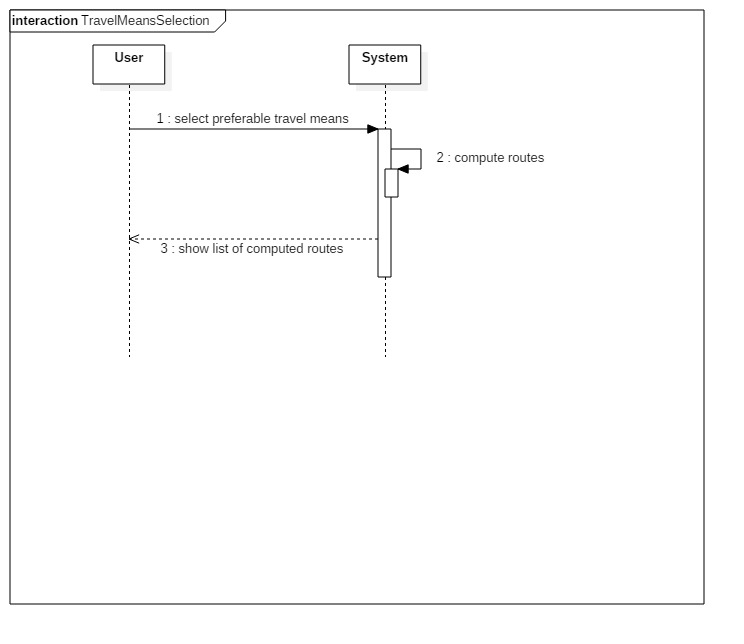
\includegraphics[scale=0.4]{TravelMeansSelection_seq_271017_1}
	\end{center}
	\caption{Choice of travel means sequence diagram}
\end{figure}
\begin{figure}[!h]
	\begin{center}
		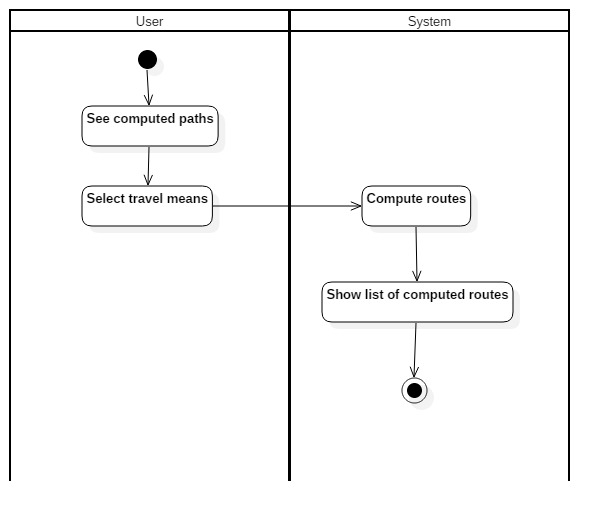
\includegraphics[scale=0.3]{TravelMeansSelection_act_271017_1}
	\end{center}
	\caption{Choice of travel means activity diagram}
\end{figure}

\newpage
\subsubsection{Use case 5.1 User (Client) selects travel means he/she wants to reach his/her destination}

 \begin{table}[!h]
 	\centering
 	\begin{tabular}{|l|l|}
 		\hline
 		Actors            & User (Client)   \\ \hline
 		Goals             &  {[}G06 {]} {[}G07{]}\\ \hline
 		Input conditions  & \begin{tabular}[c]{@{}l@{}}1. User has logged in.\\ 2. The User has the set of paths to reach his/her destination.\\ 3. User has defined his/her transport preferences.\end{tabular}            \\ \hline
 		Events flow       & \begin{tabular}[c]{@{}l@{}}1. User chooses the option “Choose transport”.\\ 2. The system shows the User a list of available routes according \\to his/her preferences in order of decreasing the suitability.\end{tabular}            \\ \hline
 		Output conditions & The User gets the set of the preferable routes.  \\ \hline
 		Exceptions        & \begin{tabular}[c]{@{}l@{}}1. There are no routes with User’s preferable travel means.\\ This exception is handled with notifying User about the issue and \\taking to Use Case 5.2.\end{tabular} \\ \hline
 	\end{tabular}
 \end{table}

\newpage
\subsubsection{Use case 5.2 User (Visitor) selects travel means he/she wants to reach his/her destination}

\begin{table}[!h]
	\centering
	\begin{tabular}{|l|l|}
		\hline
		Actors            & User (Visitor)  \\ \hline
		Goals             & {[}G03{]}  {[}G06{]} {[}G07{]}\\ \hline
		Input conditions  & The User has the set of paths to reach his/her destination. \\ \hline
		Events flow       & \begin{tabular}[c]{@{}l@{}}1. User selects the option “Choose transport".\\ 2. The system shows User the list of available travel means. \\3. User puts flags near his/her preferable travel means.\\ 4. User clicks on the “Confirm” button to save his/her choice.\\ 5. The system shows User the list of available routes according \\to his/her preferences in order of decreasing the suitability.\end{tabular}                             \\ \hline
		Output conditions & The User gets the set of the preferable routes.  \\ \hline
		Exceptions        & \begin{tabular}[c]{@{}l@{}}1. There is no User’s preferable transport.\\ This exception is handled redirecting the User to the page of \\Technical support.\\ \\ 2. User has not chosen any preferable transport.\\ The exception is handled with notifying the issue to User and \\taking back to the point 1 of Events Flow.\end{tabular} \\ \hline
	\end{tabular}
\end{table}

\newpage
\subsubsection{Use case 6 User creates a "break"}

\begin{table}[!h]
	\centering
	\begin{tabular}{|l|l|}
		\hline
		Actors            & User \\ \hline
		Goals             & {[}G04{]} {[}G13{]} \\ \hline
		Input conditions  & The User has already logged in.\\ \hline
		Events flow       & \begin{tabular}[c]{@{}l@{}}1. The system shows the User schedule of his/her meetings.\\ 2.	The User chooses a period of time between meetings.\\ 3.	The User clicks on the “Create a break” button.\\	4.	The User sets up his/her break.\\	5.	The User sets up the durability of his/her break.\\	6.	The User clicks on “Confirm” button.
		\end{tabular}  \\ \hline
		Output conditions & The User gets the break in the schedule of his/her meetings.  \\ \hline
		Exceptions        & \begin{tabular}[c]{@{}l@{}}1.	The User chooses invalid range of time given for a meeting.\\2.	The User does not choose the range of time for the break.\\All exceptions are handled with notifying the issue to the Client and taking back \\to the point 2 of Events Flow.\\ \\	3.	The User does not input any data for the break.\\The exception is handled with notifying the issue to the Client and offering to \\cancel the operation or take back to the point 4 of Events Flow. \\ \\4.	The durability of the User’s break is too long and cross with the period \\of other meetings.\\5.	The User does not set up the durability of his/her break. \\The exception 4 and 5 are handled with notifying the issue to the User and \\taking back to the point 5 of Events Flow.
		\end{tabular} \\ \hline
	\end{tabular}
\end{table}

\begin{figure}[!h]
	\begin{center}
		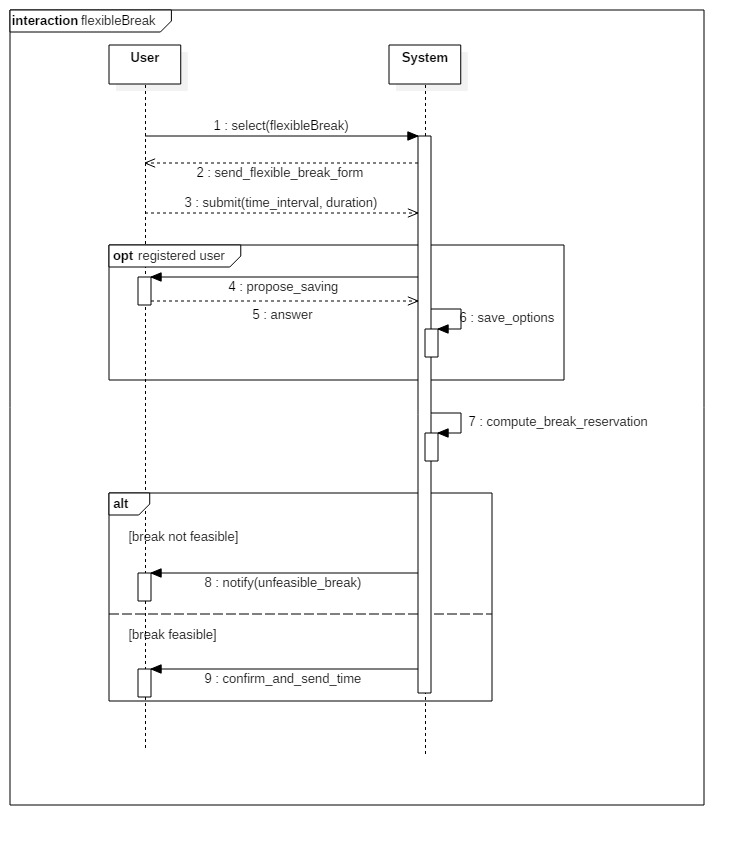
\includegraphics[scale=0.3]{Break_seq_241017_1}
	\end{center}
	\caption{Flexible break sequence diagram}
\end{figure}

\begin{figure}[!h]
	\begin{center}
		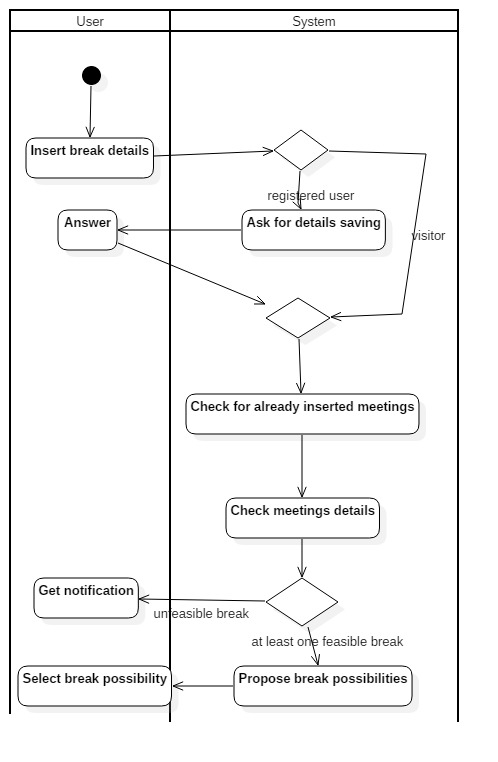
\includegraphics[scale=0.3]{Break_act_241017_1}
	\end{center}
	\caption{Flexible break activity diagram}
\end{figure}

\newpage
\subsubsection{Use case 7 User buys a ticket for the trip}

\begin{table}[!h]
	\centering
	\begin{tabular}{|l|l|}
		\hline
		Actors            & \begin{tabular}[c]{@{}l@{}}User \\ATM \\Trenord\\ Technical support
		\end{tabular}  \\ \hline
		Goals             & {[}G10{]} \\ \hline
		Input conditions  & The User selects the route with using public transport except taxi\\ \hline
		Events flow       & \begin{tabular}[c]{@{}l@{}}1.	The system offers the User to buy a ticket for his/her trip.\\2.	The User clicks on the “Confirm” button.\\3.1. If User selects a train, the system redirects him/her to Trenord site \\(“buy ticket” page).\\3.2. If User selects a bus/tram/metro, the system redirects him/her to ATM site \\(“buy ticket” page).
		\end{tabular}  \\ \hline
		Output conditions & The User buys the ticket on ATM/Trenord site.  \\ \hline
		Exceptions        & \begin{tabular}[c]{@{}l@{}}1.	The User does not want to buy a ticket. \\The exception is handled with notifying about the issue and cancelling the operation.\\2.	ATM site does not work.\\The exception is handled with User clicking on "Cancel" button and notifying to \\User and Technical Support and redirecting to the Technical Support page.
		\end{tabular} \\ \hline
	\end{tabular}
\end{table}

\begin{figure}[!h]
	\begin{center}
		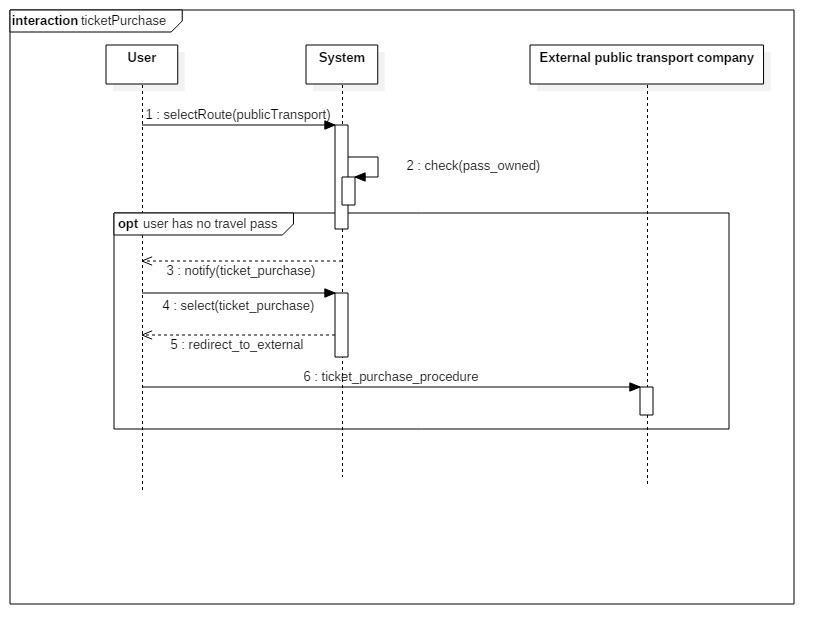
\includegraphics[scale=0.3]{Ticket_seq_241017_1}
	\end{center}
	\caption{Ticket purchase sequence diagram}
\end{figure}

\begin{figure}[!h]
	\begin{center}
		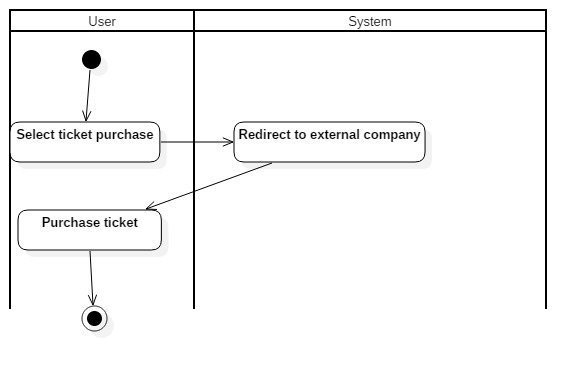
\includegraphics[scale=0.3]{Ticket_act_241017_1}
	\end{center}
	\caption{Ticket purchase activity diagram}
\end{figure}

\newpage
\subsubsection{Use case 8 User is informed about upcoming events}

\begin{table}[!h]
	\centering
	\begin{tabular}{|l|l|}
		\hline
		Actors            & User  \\ \hline
		Goals             & {[}G15{]} \\ \hline
		Input conditions  & The User has a meeting in his/her schedule.\\ \hline
		Events flow       & \begin{tabular}[c]{@{}l@{}}1.	The system computes the path time.\\ 2.	The system sets up the timer to alert the User about upcoming \\meeting in the required time.\\3.	The timer works.\\	4.	The user switches off the timer with "OK" button.			
		\end{tabular}  \\ \hline
		Output conditions & The User knows about the upcoming meeting. \\ \hline
		Exceptions        & \begin{tabular}[c]{@{}l@{}}1.	The User does not hear the alarm.\\The exception is handled with re-alerting the User in 1 minute.
			\end{tabular} \\ \hline
	\end{tabular}
\end{table}


\subsubsection{Use case 9 User activates the route}

\begin{table}[!h]
	\centering
	\begin{tabular}{|l|l|}
		\hline
		Actors            & User  \\ \hline
		Goals             & {[}G07{]} \\ \hline
		Input conditions  & The User chooses a route.\\ \hline
		Events flow       & \begin{tabular}[c]{@{}l@{}}1.	The User clicks on “Let’s go!” button.
			\\2.	The system activates the route.
			\\3.	The system activates the tracing of the User’s location.				
		\end{tabular}  \\ \hline
		Output conditions & User receives actual information about his/her motion through the route. \\ \hline
		Exceptions        & \begin{tabular}[c]{@{}l@{}}1.	The User does not want to go and clicks on “Cancel” button.  \\
			The exception is handled with notifying about the issue and \\taking back to the home page.\\
			2. The User clicks on "I have problems with the route". \\
			The exception is handled with notifying User about the issue and \\redirecting to Use case 12.
		\end{tabular} \\ \hline
	\end{tabular}
\end{table}

\newpage
\subsubsection{Use case 10 User gets information about strikes}

\begin{table}[!h]
	\centering
	\begin{tabular}{|l|l|}
		\hline
		Actors            & \begin{tabular}[c]{@{}l@{}}User\\ ATM \\ Trenord \end{tabular} \\ \hline
		Goals             & {[}G08{]} \\ \hline
		Input conditions  & The User has the set of possible paths.\\ \hline
		Events flow       & \begin{tabular}[c]{@{}l@{}}1.	The system receives information about the strike from ATM and Trenord sites.\\
			2.	The system blocks the participating public transport.\\
			3.	The User gets a notification about the strike.\\
			4.	The system shows the User available travel means.\\
			5.	The system asks the User about the continuing of the operation. \\
			6.	The User clicks on “Confirm” button.\\
			7.	The User chooses preferable travel means.\\
			8.	The User clicks on “OK” button.				
		\end{tabular}  \\ \hline
		Output conditions & The User has a set of preferable routes.\\ \hline
		Exceptions        & \begin{tabular}[c]{@{}l@{}}1.	The User chooses blocked travel means.\\
			The exception is handled with notifying about the issue to the User and \\taking back to the point 4 of Events Flow.\\ \\
			2.	The User does not want to continue the operation.\\
			The exception is handled with notifying about the issue to the User and \\taking back to the home page.			
		\end{tabular} \\ \hline
	\end{tabular}
\end{table}




\subsubsection{Use case 11  User gets information about a dangerous zone}

\begin{table}[!h]
	\centering
	\begin{tabular}{|l|l|}
		\hline
		Actors            & User \\ \hline
		Goals             & {[}G08{]} \\ \hline
		Input conditions  & The User has the set of possible paths.\\ \hline
		Events flow       & \begin{tabular}[c]{@{}l@{}}1.	The system compares the paths with the pre-defined set of risk zones.\\
			2.	If the piece of the path corresponds to one of the risk zone, the system \\sends the User a notification.\\
			3.	User clicks on “I understand!” button.\\
			4.	The system shows the User available travel means in order of increasing\\a risk.\\
			5.	The system asks the User about the continuing of the operation. \\
			6.	The User clicks on “Confirm” button.\\
			7.	The User chooses a preferable travel mean.\\
			8.	The User clicks on “OK” button.				
		\end{tabular}  \\ \hline
		Output conditions & The User has a preferable route.\\ \hline
		Exceptions        & \begin{tabular}[c]{@{}l@{}}1.	There are no risk zones in the path.\\
			The exception is handled with redirecting the User to Use Case 9.\\ \\
			2.	The User does not want to go through the risk zone.\\
			The exception is handled with notifying about the issue to the User and \\taking back to the Use case 12.	
		\end{tabular} \\ \hline
	\end{tabular}
\end{table}

\newpage
\subsubsection{Use case 12 The User gets alternative path}

\begin{table}[!h]
	\centering
	\begin{tabular}{|l|l|}
		\hline
		Actors            & User \\ \hline
		Goals             & {[}G17{]} \\ \hline
		Input conditions  & \begin{tabular}[c]{@{}l@{}}1. The User has a dangerous path.\\
		2. The User clicks on "I have problems with the route" button. 	\end{tabular}
		\\ \hline
		Events flow       & \begin{tabular}[c]{@{}l@{}}1.	The system computes a path without the risk zone.\\
			2.	The system shows the User a list of secure paths. \\
			3.	The User chooses a preferable path.\\
			4.	The User clicks on “Confirm” button.\\				
		\end{tabular}  \\ \hline
		Output conditions & The User has a preferable path. \\ \hline
		Exceptions        & \begin{tabular}[c]{@{}l@{}}1.	The User does not find a preferable path.\\
			The exception is handled with notifying the User about cancellation \\of the operation and taking back to the home page.\\ \\
			2.	There are no paths without the risk zone.\\
			The exception is handled with notifying the User about the issue and \\taking back to the Use Case 9.
		\end{tabular} \\ \hline
	\end{tabular}
\end{table}




\subsubsection{Use case 13 User reserves a bike with a bike-sharing service (Mobike)} 

\begin{table}[!h]
	\centering
	\begin{tabular}{|l|l|}
		\hline
		Actors            & \begin{tabular}[c]{@{}l@{}}User\\ Mobike\\Technical support \end{tabular} \\ \hline
		Goals             & {[}G11{]} \\ \hline
		Input conditions  & The User has a set of preferable routes.\\ \hline
		Events flow       & \begin{tabular}[c]{@{}l@{}}1.	The User chooses a bike-sharing route.\\
			2.	The system redirects the User to the map.\\
			3.	The system shows the nearest locations of bike-sharing.\\
			4.	The User chooses a preferable location.\\
			5.	The system shows the User information about a bike unlocking.\\
			6.	The User clicks on the “I understand!” button.\\
			7.	The system redirects the User to Mobike site.	
		\end{tabular}  \\ \hline
		Output conditions & The User rents the bike on Mobike site.\\ \hline
		Exceptions        & \begin{tabular}[c]{@{}l@{}}1.	The User does not find a preferable location.\\
			The exception is handled with notifying the User about cancellation \\of the operation and taking back to the Use case 5.\\ \\
			2.	Mobike site does not work.\\
			The exception is handled with notifying about the issue to the Technical \\Support and the User and redirecting the User to the Technical \\Support page.\\ \\
			3.	The User does not like the way how to unlock the bike.\\
			The exception is handled with the User’s clicking on the button \\“I don’t want” and taking back to the Use case 5.		
		\end{tabular} \\ \hline
	\end{tabular}
\end{table}


\subsubsection{Use case 14 User reserves a car with a car-sharing service (Car2Go)}

\begin{table}[!h]
	\centering
	\begin{tabular}{|l|l|}
		\hline
		Actors            & \begin{tabular}[c]{@{}l@{}}User\\ Car2Go\\ Technical support \end{tabular} 
		\\ \hline
		Goals             & {[}G12{]} \\ \hline
		Input conditions  & The User has a set of preferable routes.\\ \hline
		Events flow       & \begin{tabular}[c]{@{}l@{}}1.	The User chooses a car-sharing route.\\
			2.	The system redirects the User to the map.\\
			3.	The system shows the nearest locations of car-sharing.\\
			4.	The User chooses a preferable location.\\
			5.	The system shows the User information about a car unlocking.\\
			6.	The User clicks on the “I understand!” button.\\
			7.	The system redirects the User to Car2go site.	
		\end{tabular}  \\ \hline
		Output conditions & The User rents the car on Car2Go site.\\ \hline
		Exceptions        & \begin{tabular}[c]{@{}l@{}}1.	The User does not find a preferable location.\\
			The exception is handled with notifying the User about cancellation \\of the operation and taking back to the Use case 5.\\ \\
			2.	Car2go site does not work.\\
			The exception is handled with notifying about the issue to the Technical \\Support and the User and redirecting the User to the Technical support \\page.\\ \\
			3.	The User does not like the way how to unlock the car.\\
			The exception is handled with the User’s clicking on the button \\“I don’t want” and taking back to the Use case 5.
					\end{tabular} \\ \hline
	\end{tabular}
\end{table}

\newpage
\begin{figure}[!h]
	\begin{center}
		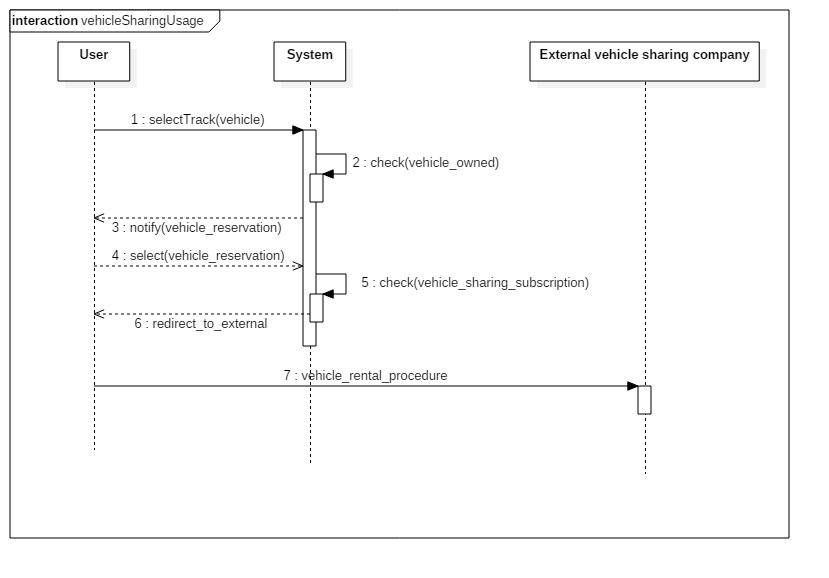
\includegraphics[scale=0.3]{VehicleSharing_seq_241017_1}
	\end{center}
	\caption{Vehicle-sharing sequence diagram}
\end{figure}

\begin{figure}[!h]
	\begin{center}
		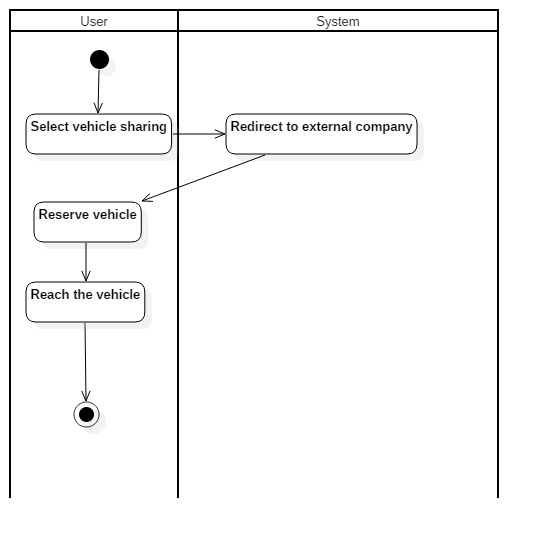
\includegraphics[scale=0.3]{VehicleSharing_act_241017_1}
	\end{center}
	\caption{Vehicle-sharing sequence diagram}
\end{figure}

\newpage
\subsubsection{Use case 15 User changes his/her route during the trip}

\begin{table}[!h]
	\centering
	\begin{tabular}{|l|l|}
		\hline
		Actors            & User \\ \hline
		Goals             & {[}G16{]} \\ \hline
		Input conditions  & The route is activated.		\\ \hline
		Events flow       & \begin{tabular}[c]{@{}l@{}}1.	The User clicks on “Change the route” button.\\
			2.	The system asks the User to confirm the pause.\\
			3.	The User clicks on “Confirm” button.\\
			4.	The system stops the route.\\
			5.	The system asks the User what he/she wants to change.\\
			5.1.1.	 If the User wants to change the meeting location, he/she \\inputs the necessary address in the field.\\
			5.1.2.	The User clicks on “Confirm” button.\\
			5.1.3.	The system computes the path.\\
			5.1.4.	The User puts a flag near a preferable travel mean in the \\list of available preferable travel means.\\
			5.2.	1. If the User wants to change a travel mean, he/she puts \\a flag near a travel mean in the list of available preferable travel means.\\
			1.2.2.	The User clicks on “Confirm” button.\\
			6.	The User clicks on “Let’s go” button.\\
			7.	The system activates a route.						
		\end{tabular}  \\ \hline
		Output conditions & The User activates the changed route. \\ \hline
		Exceptions        & \begin{tabular}[c]{@{}l@{}}1.	The User wants to take a break and he/she clicks on \\“Create a break” button.\\
			The exception is handled with redirecting to the Use Case 6. \\ \\
			2.	The User inputs the wrong address.\\
			The exception is handled with notifying about the issue to the User and \\taking back to point 5.1.1.\\ \\
			3.	The User wants to stop the route.\\
			The exception is handled with clicking on “Cancel” button, \\notifying about the issue to the User and taking back to the home page.
		\end{tabular} \\ \hline
	\end{tabular}
\end{table}

\newpage
\subsubsection{Use case 16 User chooses a preferable travel mean which is not included in the mail list}

\begin{table}[!h]
	\centering
	\begin{tabular}{|l|l|}
		\hline
		Actors            & \begin{tabular}[c]{@{}l@{}} User \\ Technical Support 	\end{tabular} \\ \hline
		Goals             & {[}G03{]} \\ \hline
		Input conditions  & The User has a set of paths.		\\ \hline
		Events flow       & \begin{tabular}[c]{@{}l@{}}1.	The User clicks on “Choose travel mean” button.\\
			2.	The User clicks on “More” button.\\
			3.	The User chooses a preferable transport in the list of extra shared \\travel means.\\
			4.	The system shows a corresponding link of the necessary site.\\
			5.	The User clicks on the link.						
		\end{tabular}  \\ \hline
		Output conditions & The User is redirected to the necessary sharing site.\\ \hline
		Exceptions        & \begin{tabular}[c]{@{}l@{}}1. There is no the necessary travel mean.\\
			The exception is handled with the User clicking on the “I want more!”\\button and redirecting him/her to the Technical support page.\\ \\
			2.	The link does not work.\\
			The exception is handled with notifying about the issue to the Technical \\Support and the User and redirecting the User to the Technical support\\page.			
		\end{tabular} \\ \hline
	\end{tabular}
\end{table}


\subsubsection{Use case 17 User uses an own car as one of the  preferable travel means}

\begin{table}[!h]
	\centering
	\begin{tabular}{|l|l|}
		\hline
		Actors            & User \\ \hline
		Goals             & {[}G03{]} \\ \hline
		Input conditions  & \begin{tabular}[c]{@{}l@{}}The User chooses a “Car” or "Bike"  option in the list of available travel\\means.\end{tabular}		\\ \hline
		Events flow       & \begin{tabular}[c]{@{}l@{}}1.1.	The system asks the User about having a private car.\\
			1.2.	The system asks the User about having a private bike. \\
			2.	The User clicks on “Confirm” button.\\
			3.	The system asks to remember his/her decision. \\
			4.	The User clicks on “Allow” button.								
		\end{tabular}  \\ \hline
		Output conditions & The User has a route by his/her own car or bike.\\ \hline
		Exceptions        & \begin{tabular}[c]{@{}l@{}}1.	The User does not have a private car.\\
			The exception is handled with offering the User “taxi” or “car-sharing”\\option.\\
			1.	The User does not have a private bike.\\
			The exception is handled with offering the User “bike-sharing” option.\\
			2.	The User does not want the system to remember his/her choice.\\
			The exception is handled with clicking on “Don’t allow” button.
		\end{tabular} \\ \hline
	\end{tabular}
\end{table}


\newpage
\subsubsection{Use case 18 User creates a meeting}

\begin{table}[!h]
	\centering
	\begin{tabular}{|l|l|}
		\hline
		Actors            & User \\ \hline
		Goals             & {[}G14{]} \\ \hline
		Input conditions  & The User creates a meeting.	\\ \hline
		Events flow       & \begin{tabular}[c]{@{}l@{}}1.	The User clicks on 'Create a meeting" button.\\
			2.	The User fills information about the meeting in the corresponding fields.\\
			3.	The User selects a priority of the meeting (1-business, 2-appointment, 3-with\\friends, 4-personal).				
			4. The User clicks on "Confirm" button.						
		\end{tabular}  \\ \hline
		Output conditions & The User has a meeting in his/her schedule.\\ \hline
		Exceptions        &  \begin{tabular}[c]{@{}l@{}} 1.	The User does not choose the priority of the meeting.\\
			The exception is handled with setting priority 1 of the meeting by default.\\
			2.	The User does not input information about the meeting.\\
			The exception is handled with notifying the issue to the User and taking back \\to the point 2 of Events Flow.
			2.	The User does not want to create the meeting\\any more.\\
			The exception is handled with User clicking on "Cancel" button and taking back \\to the home page.
			\end{tabular}\\ \hline
	\end{tabular}
\end{table}

\begin{figure}[!h]
	\begin{center}
		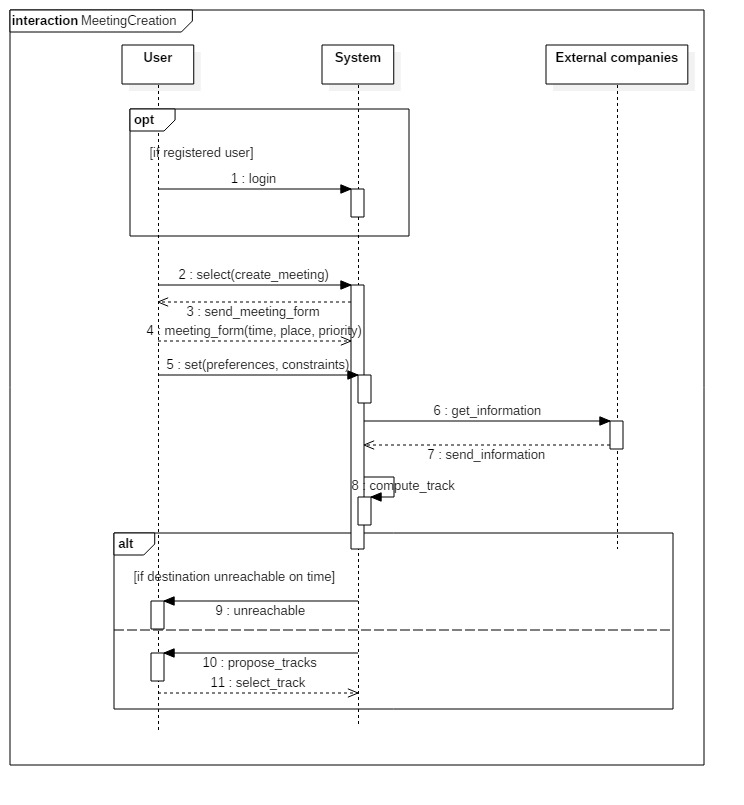
\includegraphics[scale=0.3]{sequenceDiagram_MeetingCreation_231017_1}
	\end{center}
	\caption{Meeting creation sequence diagram}
\end{figure}

\begin{figure}[!h]
	\begin{center}
		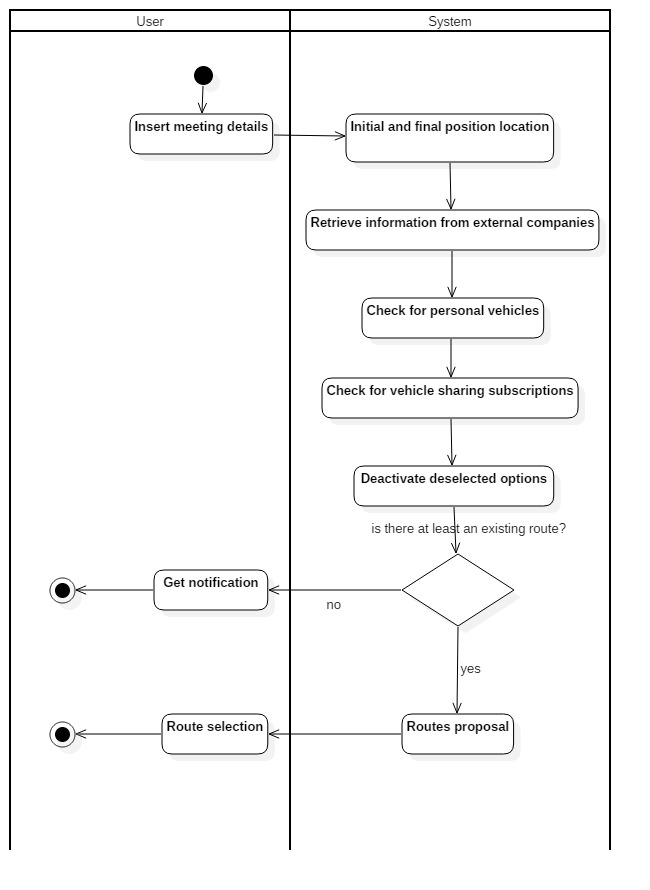
\includegraphics[scale=0.3]{meetingCreation_act_281017_1}
	\end{center}
	\caption{Meeting creation activity diagram}
\end{figure}
\newpage
\subsubsection{Use case 19 User is out of time for the meeting}

\begin{table}[!h]
	\centering
	\begin{tabular}{|l|l|}
		\hline
		Actors            & User \\ \hline
		Goals             & {[}G05{]} \\ \hline
		Input conditions  & The User creates a meeting.	\\ \hline
		Events flow       & \begin{tabular}[c]{@{}l@{}}1.	The system computes the shortest required time to reach the \\destination.\\
			2.	The system compares the shortest required time and the time left \\for the meeting.\\
			3.	If the time the User has is less than the shortest required time, \\the system notifies the User about the lack of time.										
		\end{tabular}  \\ \hline
		Output conditions & The User has a warning about unreachable time.\\ \hline
		Exceptions        & \\ \hline
	\end{tabular}
\end{table}

\newpage
\subsubsection{Use case 20 Technical support fixes problems with redirecting to external company}

\begin{table}[!h]
	\centering
	\begin{tabular}{|l|l|}
		\hline
		Actors            & Technical support\\ \hline
		Goals             & {[}G10{]} \\ \hline
		Input conditions  & \begin{tabular}[c]{@{}l@{}}1.	The Technical support has logged in.\\
		2.	The Technical support receives the notification about the issue \\with redirecting to a site.
	\end{tabular}\\ \hline
		Events flow       & \begin{tabular}[c]{@{}l@{}}1.	The Technical support sends a query to the database with additional \\links to similar sites without API providing.\\
			2.	The Technical support selects a link of a corresponding site.\\
			3.	The Technical support replaces broken link with a page with apologizes \\and the link.													
		\end{tabular}  \\ \hline
		Output conditions & The system has a working link.\\ \hline
		Exceptions        &  \\ \hline
	\end{tabular}
\end{table}


\subsubsection{Use case 21 User selects the most ecological route}

\begin{table}[!h]
	\centering
	\begin{tabular}{|l|l|}
		\hline
		Actors            & User\\ \hline
		Goals             & {[}G18{]} \\ \hline
		Input conditions  & The User has a set of preferable routes.\\ \hline
		Events flow       & \begin{tabular}[c]{@{}l@{}}1.	The system selects the route by foot, by bike or by using bike-sharing service.\\
			2.	The system defines these routes as the most ecological route.\\
			3.	The system offers the User the most ecological route.\\
			4.	The User clicks on “I choose this route!”										
		\end{tabular}  \\ \hline
		Output conditions & The User has a preferable route.\\ \hline
		Exceptions        & \begin{tabular}[c]{@{}l@{}} 1.	The User does not want to use the most ecological route.\\
		The exception is handled with User clicking on “I don’t want” button and \\showing the list of the other possible routes.\end{tabular} 
		\\ \hline
	\end{tabular}
\end{table}

\newpage
\subsubsection{Use case 22 User gets information about weather conditions}

\begin{table}[!h]
	\centering
	\begin{tabular}{|l|l|}
		\hline
		Actors            & \begin{tabular}[c]{@{}l@{}}User \\ Weather forecast site (meteo.it) \end{tabular} \\ \hline
		Goals             & {[}G09{]} \\ \hline
		Input conditions  & The User has a set of preferable routes.\\ \hline
		Events flow       & \begin{tabular}[c]{@{}l@{}}1.	The system addresses a query of the nearest weather forecast to Weather \\forecast site providing us API.\\
			2.	The system gets the information about the nearest weather forecast. \\
			3.	If it rains or snows during the User’s trip, the system blocks unsuitable \\travel means (bike-sharing, bike, walking).\\
			4.	The system warns the User about the bad weather conditions.\\
			1.	The User clicks on “OK” button.\\
			2.	The User selects a preferable travel mean in the list of available travel means.												
		\end{tabular}  \\ \hline
		Output conditions & The User has a preferable route.\\ \hline
		Exceptions        & \begin{tabular}[c]{@{}l@{}} 1.	The User does not want to go to the meeting when the weather is bad.\\
			The exception is handled with User clicking on “Cancel trip”, confirming his/her \\decision and taking back to the home page.
		\end{tabular} 
		\\ \hline
	\end{tabular}
\end{table}


\subsection{Traceability matrix}
\begin{tabular}{|c|c|c|c|}
	\hline 
	\textbf{Goal ID}&  \textbf{Req ID}& \textbf{Use Case ID} & \textbf{Comments} \\ 
	\hline  \hline
	G01& RE01, RE02, RE03, RE04, RE05 &  UC.1, UC.2&  \\ 
	\hline 
	G02&  RE08, RE09& UC.3 &  \\ 
	\hline 
	G03& RE10, RE11, RE15& UC.4, UC.5.2, UC.16, UC.17   &  \\ 
	\hline 
	G04& RE12, RE16, RE20 & UC.6 &  \\ 
	\hline 
	G05&  RE14& UC.19 &  \\ 
	\hline 
	G06&  RE17 & UC.5.1, UC.5.2  &  \\ 
	\hline 
	G07&  RE19& UC.5.1, UC.5.2, UC.9  &  \\ 
	\hline 
	G08&  RE18, RE21, RE22 &  UC.10, UC.11 &  \\ 
	\hline 
	G09& RE18  & UC.22 &  \\ 
	\hline 
	G10& RE07 & UC.7, UC.20&  \\ 
	\hline 
	G11&  RE07, RE11 & UC.13 &  \\ 
	\hline 
	G12& RE07, RE11 & UC.14 &  \\ 
	\hline 
	G13& RE13 & UC.13 &  \\ 
	\hline 
	G14&  RE23, RE24& UC.18  &  \\ 
	\hline 
	G15& RE25 & UC.8 &  \\ 
	\hline 
	G16& RE08, RE11& UC.15 &  \\ 
	\hline 
	G17& RE15, RE17 & UC.12 &  \\ 
		\hline 
	G18& RE19 & UC.21 &  \\ 
	\hline 
\end{tabular} 


\newpage
\section{Performance Requirements}
\begin{itemize}
\item (PR01): The application should calculate the path in the minimum time required.
\item (PR02): The application should use the minimum RAM space required.
\item (PR03): The application should use the minimum disk space required.
\item (PR04): The application GUI should be fluid.
\end{itemize}

\section{Design Constraints}
\subsection{Standard compliance}
\begin{itemize}
\item (SC01): The application must provide multiple languages settings (at least, English and Italian).
\item (SC02): The application should provide facilities for disable users (like High/low contrast GUI ...).
\item (SC03): The application should reserve the majority of the screen to the travel form in case of journey setup.
\item (SC04): The application should reserve the majority of the screen to the navigator in case of navigation mode.
\item (SC05): All the information that is not important in a certain moment must be stored in menus.
\item (SC06): The link for external companies must be stored in the external company area inside our application.
\item (SC07): The warnings must occupy the minimum required screen space  when they don't cause a delay that can jeopardise the journey.
\item (SC08): The warnings must occupy the entire screen space required when they cause an excessive delay.
\end{itemize}

\subsection{Hardware Limitations}
\begin{itemize}
\item (HL01): We must provide the best GUI according to the user settings and user's device.
\item (HL02): If the user's device doesn't allow some settings we cannot know it .
\end{itemize}

\subsection{Any Other Constraints}
\begin{itemize}
\item (OC01): The application must not blink for no causing epilectic disease.
\item (OC02): The application fonts must be big enough to be read by the user.
\end{itemize}

\section{Software System Attributes}

\subsection{Reliability}
\begin{itemize}
\item (RR01): The application must be able to calculate alternatives in case of problems during the journey
\item (RR02): The application should retrieve the most updated information from the external sites.
\item (RR03): The application should run in every mobile device with a screen which satisfies minimum requirements according to the OS of the device.
\item (RR04): In case of excessive delays the application should provide an alternative way.
\item (RR05): The application should maintain the last status in case of unexpected exit from the application.
\item (RR06): The application should run also in case of non full screen mode.
\end{itemize}

\subsection{Availability}
\begin{itemize}
\item (AR01): The application must be able to work when the Internet connection is established.
\item (AR02): The application must be able to work when it's running.
\item (AR03): The application must be able to work whit all the settings provided.
\item (AR04): The application must be able to reschedule paths in case of problems.
\end{itemize}

\subsection{Security}
\begin{itemize}
\item (SR01): The journey set by a user must be visible only by the user himself.
\item (SR02): The private area of a client should be available only fot the client himself.
\item (SR03): The data stream from the application and the user's device must be encripted.
\item (SR04): Every user must have a dedicated thread, not shared with other users.
\item (SR05): The application should not manage too sensible user's data.
\end{itemize}

\subsection{Maintainability}
\begin{itemize}
\item (MR01): The software must use as much as possible interfaces in order to have a "contract" for future features.
\item (MR02): The software must use the standard Java version (8.0 or later).
\item (MR03): The external libraries must be provided by external big companies (like Google, Twitter ...)
\item (MR04): The software releases must be provided with documentation related.
\item (MR05): The software must be commented in all the important parts using JavaDocs comments.
\item (MR06): All the public aspects of the software must be available in every next versions (if necessary they can be deprecated but not deleted).
\end{itemize}

\subsection{Portability}
\begin{itemize}
\item (PtR01): The application should use Java only server side.
\item (PtR02): The application should use less native languages as possible.
\item (PtR03): The application should rely on standards (HTML5, CSS, JSon ...)in order to provide almost the same user experience in all the possible devices.
\end{itemize}

\chapter{FORMAL ANALYSIS USING ALLOY}

\section{Script of the model}

\begin{lstlisting}

module TravalendarPlus/Signatures

open util/integer

/** ===================={ Preliminary Notes }==================== **/
/* In these Signatures we have avoided to define attributes that are not 
important (e.g. Id ,title, ...) to show the connection between the objects of our 
application (but that could be important in the final development of the
application). This choice was done primarly to semplify the final view of the
Graph and to focus only on connections between our classes instances.
*/

/** ===================={ Coordinate Signature }==================== **/
sig Coordinate{
latitude: Int,
longitude: Int
}{
latitude > 0 && longitude > 0
}

/** ===================={ UserDeviceAdapter Signature }==================== **/
/* This signature corresponds to an interface , which defines methods and
attributes that are necessessary to interract with the device'os of the user in a
uniformed way.*/
abstract sig UserDeviceAdapter{}

sig IOSDeviceAdapter extends UserDeviceAdapter{}
sig AndroidDeviceAdapter extends UserDeviceAdapter{}
sig WindowsPhoneDeviceAdapter extends UserDeviceAdapter{}

/** ===================={ User Signature }==================== **/
abstract sig User {
deviceAdapter: one UserDeviceAdapter,
--This attribute is used to keep track of the actual localization of the
user without having to create a meeting
actualCoordinate: one Coordinate,
scheduledMeetings: disj set Meeting
}

sig Visitor extends User {}
/* At this initial stage of the development of our application there is
no distinction between a client and a visitor*/
sig Client extends User {}

/** ===================={ MeanOfTransport Signature }==================== **/

abstract sig MeanOfTransport {
--This attribute is used to store the current location of a mean of
transport if it's provided
location: lone Coordinate
}

sig Feet extends MeanOfTransport{}
sig Bike extends MeanOfTransport{}
sig Boat extends MeanOfTransport{}
/*(Other Non Autonomous Means Of Transport) This class is used to provide
a flexible way to define another mean of
transport (without an engine)that was not defined before*/
sig ONAMOT extends MeanOfTransport{}

sig Car extends MeanOfTransport{}
sig Tram extends MeanOfTransport{}
sig Ship extends MeanOfTransport{}
sig Bus extends MeanOfTransport{}
sig Train extends MeanOfTransport{}
sig Taxi extends MeanOfTransport{}
/*(Other Autonomous Means Of Transport) This class is used to provide
a flexible way to define another mean of transport (whit an engine) that
was not defined before*/
sig OAMOT extends MeanOfTransport{}

/** ===================={ Path Restriction Signature }==================== **/
/* This signature corresponds to a TripRestriction interface whose purpose
is to define a standard notation for adding possible restriction in which
the user can occur during his trip.*/
abstract sig PathRestriction{}

/* Restriction associated to the license required for passing through a
specific path */
sig LicenceRestriction extends PathRestriction {}
/* Restriction  associated to the carbon footprint emissions for passing through
a specific path*/
sig EuroRestriction extends PathRestriction {}
/* Restriction associated to a size required for passing through a specific path*/
sig SizeRestriction extends PathRestriction {}
/* Restriction  associated to a generic restriction for passing through a specific
path.*/
sig OtherRestriction extends PathRestriction{}

/** ===================={ Break Signature }==================== **/
sig Break{}

/** ===================={ Trip Signature }==================== **/
sig Trip {
startingPoint: one Coordinate,
endingPoint: one Coordinate,
break: lone Break,
nextTrip: lone Trip,
previousTrip: lone Trip,
pathRestrictions: disj set PathRestriction,
meanOfTransport: one MeanOfTransport,
--This attribute is used to design the map in the user's screen
navigator: one Navigator,
startingTime: one Time,
endingTime: one Time
}

/** ===================={ Meeting Signature }==================== **/
sig Meeting {
trips: disj set Trip,
startingTime: one Time,
endingTime: one Time
}

/** ===================={ Notification Signature }==================== **/
/* This signature corresponds to an interface , which defines methods and attributes
that are necessary have a standardized  notification that can be used to aware
the user about some problems or information.*/
abstract sig Notification{}

sig StrikeNotification extends Notification {
relatedCompany:one ExternalMeanOfTransportCompany
}

sig WeatherNotification extends Notification{
relatedCompany:one ExternalCompany,
-- used to define which users of our application are affected by this notifications
affectedWalkers:disj set Feet,
-- used to define which bikers of our application are affected by this
notifications
affectedBikers:disj set Bike,
}

/* This class is used to alert the user about other kind of problems or
information (like intense traffic )*/
sig OtherNotification extends Notification{
relatedCompany:one ExternalCompany
}

/** ===================={ NotificationManager Signature }==================== **/
/* Class which provides a way to inform other classes about some problems
that can occur and that have been notified*/
one sig NotificationManager{
activeNotifications: disj set Notification
}

/** ===================={ ExternalCompany Signature }==================== **/
sig ExternalCompany {}

/** =============={ ExternalMeanOfTransportCompany Signature }============== **/

sig ExternalMeanOfTransportCompany extends ExternalCompany{
meanOfTransportProvided: disj set MeanOfTransport
}

/** ===================={ Navigator Signature }==================== **/
/* This signature corresponds to a class that render the map on the user
device*/
sig Navigator {}


/** ===================={ Technician Signature }==================== **/
sig Technician{}

/** ===================={ TechnicalProblem Signature }==================== **/
sig TechnicalProblem {
user: one User,
technicians: disj set Technician
}

/** ===================={ SystemShared Signature }==================== **/
/* This singleton class contains all the information that must be shared
among all the objects of the system*/
sig SystemShared {
externalCompanies: disj set ExternalCompany,
clientsList: disj set Client,
activeVisitors: disj set Visitor,
activeClients: disj set Client,
unsolvedProblems: disj set TechnicalProblem,
solvedProblems: disj set TechnicalProblem,
notificationManager: one NotificationManager,
techniciansList: disj set Technician,
activeTechnicians: disj set Technician
}

/** ===================={ Time Signature }==================== **/
sig Time {
--Attribute associated to hours
h: Int,
--Attribute associated to minutes
m: Int
}{
h >= 0 && h < 24 && m >= 0 && m < 60
} 

/** ===================={ Coordinate Axioms }==================== **/

--1)Coordinates cannot be free , they must be related to some objects
fact allCoordinatesAreBinded{
all c: Coordinate |
((c in User.actualCoordinate)|| (c in Trip.startingPoint) ||
(c in Trip.endingPoint)|| (c in MeanOfTransport.location))
}

--2)No shared coordinates between different kinds of objects
fact noSharedCoordinatesBetweenUsers{
all disj u1,u2: User | u1.actualCoordinate != u2.actualCoordinate }
fact noSharedCoordinatesTripsAndUsers1{	
all u: User |all  t: Trip | u.actualCoordinate != t.startingPoint}

//The instances of coordinates aren't shared between the user position and the trip
ending point
fact noSharedCoordinatesTripsAndUsers2{
all u: User |all  t: Trip |u.actualCoordinate != t.endingPoint }
fact noSharedCoordinatesBetweenMeanOfTransports{ 
all disj m1,m2: MeanOfTransport | m1.location != m2.location }
fact noSharedCoordinatesBetweenMeanOfTransportsAndUsers{
all u: User | all m: MeanOfTransport | u.actualCoordinate != m.location }
fact noSharedCoordinatesBetweenMeanOfTransportAndTripStartingPosition{
 all t: Trip | all m: MeanOfTransport |
(m.location != t.startingPoint) && (m.location != t.endingPoint)  }

--3)Each trip must be associated to different instances of coordinate from other
trips
fact eachTripHasItsCoordinate{
all disj t1, t2: Trip |
(t1.startingPoint != t2.startingPoint) && (t1.endingPoint != t2.endingPoint)
}

--4)Trips that are in a sequence has related coordinates
fact relatedCoordinates{ all disj t1, t2: Trip |
(t1.startingPoint = t2.endingPoint) <=> ((t1 = t2.nextTrip)&&
(t2 = t1.previousTrip))
}

--5)Each MeanOfTransport must be associated to different instances of
coordinate from other MeanOfTransport
fact eachMeanOfTransportHasItsCoordinate{ 
all disj m1, m2: MeanOfTransport | m1.location != m2.location}

--6)Each coordinates has different values of latitude and longitude
fact eachCoordinateIsDifferent{ 
all disj c1,c2: Coordinate| (c1.latitude != c2.latitude) and 
(c1.longitude != c2.longitude)}

/** ===================={ User Axioms }==================== **/

--1)Each user must be associated to a different UserDeviceAdapter
fact oneUserOneDeviceAdapter{ 
all disj u1, u2: User | u1.deviceAdapter != u2.deviceAdapter }

--2)Each user must be associated to a different Meetings list
fact differentMeetingsForDifferentUsers{ 
all disj u1, u2: User | u1.scheduledMeetings != u2.scheduledMeetings }

/** ===================={ SystemShared Axioms }==================== **/
--1)There is only one instance of SystemShared
fact singletonSystemShared { no ss1, ss2: SystemShared | ss1 != ss2 }

--2)All the users of the application must be inside the system shared 
class
fact noUserOutsideSystemShared{all u: User |
(( u in SystemShared.clientsList ) ||
 (u in SystemShared.activeClients ) || 
 (u in SystemShared.activeVisitors)) }

--3)If a Client is in the active list it is also in the client list
fact activeClientAreClient{ 
all c: Client | (c in SystemShared.activeClients) => 
(c in SystemShared.clientsList) }

--4)All external companies are contained in the system shared
fact noExternalCompanyOutsideSystemShared{ 
SystemShared.externalCompanies = ExternalCompany }

--5)All technical problems must be contained in the system shared
fact noTechnicalProblemOutsideSystemShared{
((SystemShared.unsolvedProblems = TechnicalProblem) || 
(SystemShared.solvedProblems = TechnicalProblem))
}

--6)There are no problems that are both in solved and unsolved problems
fact noSolvedUnsolvedProblems{
all p: TechnicalProblem |
(((p in SystemShared.solvedProblems) => (p not in SystemShared.unsolvedProblems)) 
&& ((p in SystemShared.unsolvedProblems) => 
(p not in SystemShared.solvedProblems)))
}

--7)NotificationManager is contained in SystemShared
fact noNotificationManagerOutsideSystemShared{
SystemShared.notificationManager =  NotificationManager}

--8)All technicians are contained in the SystemShared
fact allTechniciansAreInTheSystemShared{
((SystemShared.techniciansList = Technician) ||
 (SystemShared.activeTechnicians = Technician))
}

--9)If a Technician is in the active list it is also in the technician list
fact activeTechniciansAreTechnicians{
all t: Technician| (t in SystemShared.	activeTechnicians) => 
(t in SystemShared.techniciansList)
}

--10)Meetings are only related to clients and visitors that are in the active list
fact meetingsOnlyForActiveClients{
all c: Client | ((c not in SystemShared.activeClients) => 
(c.scheduledMeetings = none))
}

fact meetingsOnlyForActiveVisitors{
all v: Visitor | ((v not in SystemShared.activeVisitors) => 
(v.scheduledMeetings = none))
}

/** ===================={ Notification Axioms }==================== **/
--1)All notifications must be related to the notification manager
fact noFreeNotifications{ 
all n: Notification | (n in NotificationManager.activeNotifications) }

--2)Weather notifications cannot be related to weather companies
fact weatherNotificationToExternalCompaniesOnly{
WeatherNotification.relatedCompany != ExternalMeanOfTransportCompany}

--3)Walkers must be notificated in case of WeatherNotifications
fact weatherNotificationsForWalkers{	
(WeatherNotification.affectedWalkers = Feet)}

--4)Bikers must be notificated in case of WeatherNotifications
fact weatherNotificationsForBikers{	
(WeatherNotification.affectedBikers = Bike)}

/** ===================={ PathRestriction Axioms }==================== **/
--1)There are no PathRestriction that are not related to a Trip
fact noFreePathRestriction{ Trip.pathRestrictions = PathRestriction }

/** ===================={ Break Axioms }==================== **/
--1)There are no breaks that are not related to a Trip
fact noFreeBreaks{ Trip.break = Break }

--2)Each Trip has a different break
fact differentTripsDifferentsBreaks{ 
all disj t1, t2: Trip | t1.break != t2.break }

/** ===================={ Meeting Axioms }==================== **/
--1)We cannot have Meetings that are not related to a User
fact noFreeMeetings{ User.scheduledMeetings = Meeting }

--2)Different meetings cannot have the same Trips
fact differentMeetingsDifferentPaths{
all disj m1,m2: Meeting | m1.trips != m2.trips}

--3)We cannot have Meetings whitout Trips
fact noFreeTripMeetings{ no m: Meeting | m.trips = none }

--4)Each meeting has it's own trips
fact noSharedTripsBetweenDifferentMeetings{
all disj m1, m2: Meeting | m1.trips.*nextTrip != m2.trips.*nextTrip}

--5)Trips transitive clojure
fact tripTransitiveClojure{
all t: Trip | all m: Meeting | ((t in m.trips) => 
((t.*nextTrip in m.trips) && (t.*previousTrip in m.trips)))}

--6)Correct time sequence in meetings
fact correctMeetingTimeSequence{
all m1: Meeting|all disj t1,t2: Trip |
((t1 in m1.trips) && (t2 in m1.trips) && (t1.previousTrip = none) &&
(t2.nextTrip = none)) => ((m1.startingTime.h = t1.startingTime.h) && 
(m1.startingTime.m = t1.startingTime.m) && 
(m1.endingTime.h = t2.endingTime.h) && (m1.endingTime.m = t2.endingTime.m))
}

/** ===================={ MeanOfTransport Axioms }==================== **/
--1)There are no MeanOfTransport that are not in a Trip or in an 
ExternalMeanOfTransportCompany
fact noFreeMeanOfTransport{ all m: MeanOfTransport |
((m in Trip.meanOfTransport) || 
(m in ExternalMeanOfTransportCompany.meanOfTransportProvided))}

--2)Feet are not in ExternalMeanOfTransportCompany
fact feetsCannotBeExternalized{
all f: Feet | (f not in ExternalMeanOfTransportCompany.meanOfTransportProvided)}

--3)Some MeanOfTransport must be ExternalMeanOfTransport
fact noStrangeMeanOfTransport{
all c: Taxi |all s: Ship | all t: Tram | all b: Bus | all r: Train |
((c in ExternalMeanOfTransportCompany.meanOfTransportProvided) &&
(s in ExternalMeanOfTransportCompany.meanOfTransportProvided) &&
(t in ExternalMeanOfTransportCompany.meanOfTransportProvided) &&
(b in ExternalMeanOfTransportCompany.meanOfTransportProvided) &&
(r in ExternalMeanOfTransportCompany.meanOfTransportProvided))
}

--4)If a bike is not associated to an external mean of transport it cannot be
shared
fact noSharedPresonalBikes{
all b: Bike|all disj t1,t2: Trip|
(b not in ExternalMeanOfTransportCompany.meanOfTransportProvided) => (
(t1.meanOfTransport = b) => (t2.meanOfTransport != b))
}

--5)If a car is not associated to an external mean of transport it cannot be shared
fact noSharedPresonalCar{
all b: Car|all disj t1,t2: Trip|
(b not in ExternalMeanOfTransportCompany.meanOfTransportProvided) => (
(t1.meanOfTransport = b) => (t2.meanOfTransport != b))
}

--6)Feet cannot be shared
fact noSharedFeet{
all f: Feet|all disj t1,t2: Trip| (t1.meanOfTransport = f) => 
(t2.meanOfTransport != f)}

/** ===================={ Trip Axioms }==================== **/
--1)All the trips must be contained in meetings
fact noFreeTrips{all t: Trip | (t in Meeting.trips)}

--2)No previousTrip= nextTrip
fact noPreviousNextTrip{all t: Trip| t.nextTrip != t.previousTrip}

--3)The starting point of a Trip must be different from his ending point
fact noStartingEndingPoint{no t: Trip| t.startingPoint = t.endingPoint }

--4)A trip cannot be recursive (mark it's successor/precessor as itself
fact noRecursiveTrip1{no t: Trip| (t.nextTrip = t)}
fact noRecursiveTrip2{no t: Trip| (t.previousTrip = t) }

--5)If a trip is marked as the next trip of another, this other trip must
be marked as the previous
fact correctTripSequence{all disj t1, t2: Trip | (t1.nextTrip = t2) <=> 
(t2.previousTrip = t1)}

--6)We cannot have trips that are related to anchestor trip, only
with parent
fact noPreviousTripCycles{ 
all t1,t2: Trip| (t1.*previousTrip = t2.*previousTrip) <=> (t1 = t2)	}

--7)We cannot have trips that are related to nepheus trip, only with
parent
fact noNextTripCycles2{ all t1,t2: Trip| (t1.*nextTrip = t2.*nextTrip) <=> 
(t1 = t2)}

--8)Some trip should not have next trip associated
fact someFinalTrip{some t: Trip | t.nextTrip = none}

--9)Some trip should not have previous trip associated
fact someRootTrip{some t: Trip | t.previousTrip = none}

--10)Correct time sequence in linked trips
fact correctTimeSquence1{ all t1, t2: Trip |
(t1.nextTrip = t2) => ((t1.endingTime.h = t2.startingTime.h) &&
 (t1.endingTime.m = t2.startingTime.m) )
}

fact correctTimeSquence2{ all t1, t2: Trip |
(t1.nextTrip = t2) => (
(t1.endingTime.h <= t2.endingTime.h) && (t1.endingTime.m <= t2.endingTime.m) )
}

--11)Each trip must have a starting time which is smaller than the ending
time
fact beforeStartingThanEnding{
all t: Trip |
((t.startingTime.h = t.endingTime.h) =>
(t.startingTime.m < t.endingTime.m)) || 
((t.startingTime.m = t.endingTime.m) =>(t.startingTime.h < t.endingTime.h))
}

/** ===================={ Navigator Axioms }==================== **/
--1)We cannot have navigators that are not releted to trips
fact noFreeNavigator{ Trip.navigator = Navigator }

--2)Each trip has it's own navigator
fact noSharedNavigators{
 all disj t1,t2: Trip | t1.navigator != t2.navigator}

/** ==============={ ExternalMeanOfTransportCompany Axioms }=============== **/
--1)We cannot have two different external company that have the same mean
of transport
fact noSharedExternalMeanOfTransport{
all disj ec1, ec2: ExternalMeanOfTransportCompany |
ec1.meanOfTransportProvided != ec2.meanOfTransportProvided
}

--2)All external MeanOfTransport company must have, at least, one transport 
provided
fact noEmptyExternalMeanOfTransportCompany {
all e: ExternalMeanOfTransportCompany | e.meanOfTransportProvided != none
}

--3)If a strike notification is associated to a mean of transport all trips cannot
use that mean of transport
fact noUsersThatUseStrikedMeanOfTransport{
all m: MeanOfTransport | all t: Trip | all s: StrikeNotification | 
all e: ExternalMeanOfTransportCompany|
(s.relatedCompany = e) => ((m in e.meanOfTransportProvided) => (
(t.meanOfTransport != m)))
}

/** ===================={ UserDeviceAdapter Axioms }==================== **/
--1)We cannot have UserDeviceAdapter that are not related to a User
fact noFreeUserDeviceAdapter{ User.deviceAdapter = UserDeviceAdapter }

/** ===================={ TechnicalProblem Axioms }==================== **/
--1)Each technical problem that is marked has solved must have , at last, one
technician associated
fact techniciansForSolvedProblems{
all p: TechnicalProblem | (p in SystemShared.solvedProblems) => 
(p.technicians != none)}


/** ===================={ User Assertions }==================== **/
--1)There could be users that doesn't have meetings associated
assert usersWithoutMeetings{some u: User | u.scheduledMeetings = none}

/** ===================={ MeanOfTransport Assertions }==================== **/
--1)There could be means of transport that all not related to any trip
assert unusedMeansOfTransport{
 some m: MeanOfTransport | (m not in Trip.meanOfTransport)}

--2)Means of transport that are associated to an external mean of transport company 
can be shared
assert someSharedPublicTransport{
some m: MeanOfTransport | some e: ExternalMeanOfTransportCompany| 
some disj t1, t2: Trip| (m = e.meanOfTransportProvided ) => (
(m = t1.meanOfTransport) && (t1.meanOfTransport = t2.meanOfTransport))
}

/** ===================={ PathRestriction Assertions }==================== **/
--1)There could be shared path restrictions (because some trips can pass
in same paths)
assert sharedPathRestriction{
 some disj t1,t2: Trip | (t1.pathRestrictions = t2.pathRestrictions) }

/** ===================={ Meeting Assertions }==================== **/
--1)There is always a trip of a meeting which has no previous path
associated (head of the meeting)
assert thereIsAlwaysARootTripForEachMeeting{
one t: Trip | all m: Meeting |
(t.previousTrip = none) && (t in m.trips)
}

--2)There is always a trip of a meeting which has no next path associated
(final trip of the meeting)
assert thereIsAlwaysAFinalTripForEachMeeting{
one t: Trip | all m: Meeting |
(t.nextTrip = none) && (t in m.trips)
}

/** ===================={ Notification Assertions }==================== **/
--1)Not all public mean of transport will be disabled in case of a strike
assert publicMeanOfTransportAvailabilityInCaseOfStrike{
some m: MeanOfTransport | all t: Trip | all s: StrikeNotification | 
all e: ExternalMeanOfTransportCompany| (s.relatedCompany = e) => (
(m not in e.meanOfTransportProvided) => (
(t.meanOfTransport = m)))
}

--2)Public bike won't be disabled in case of adverse weather notification
assert publicBikeAvailabilityInCaseOfWeather{
some b: Bike | all t: Trip | all w: WeatherNotification | 
all e: ExternalMeanOfTransportCompany| (w.relatedCompany = e) => (
(b in e.meanOfTransportProvided) => (
(t.meanOfTransport = b)))
}

/** ===================={ SystemShared Assertions }==================== **/
--1)There could be some unsolved technical problems that are not
associated to a technician (yet)
assert freshProblems{	some t: TechnicalProblem|
(t in SystemShared.unsolvedProblems) && (t.technicians = none)
}

/** ===================={ SystemShared Predicates }==================== **/
--1)When a problem is solved it's moved in the solvedProblemsList
pred problemsFromUnsolvedToSolved[p: TechnicalProblem, s,s': SystemShared]
{ p in s.unsolvedProblems and p.technicians != none
implies
s'.unsolvedProblems = s.solvedProblems - p and 
s'.solvedProblems = s.solvedProblems + p
}

/** ===================={ Meeting Predicates }==================== **/
--1)If a new meeting has been created by a user it must be added to the user's
scheduled meetings list
pred createAMeeting[u, u': User , m: Meeting]{
 u'.scheduledMeetings = u.scheduledMeetings + m }
pred deleteMeeting[u, u': User , m: Meeting]{
 u'.scheduledMeetings = u.scheduledMeetings - m }

--2)How to add and delete trips from meetings
pred addATrip[m,m':Meeting, nt: Trip]{ m'.trips = m.trips + nt}
pred deleteATrip[m,m':Meeting, nt: Trip]{  m'.trips = m.trips - nt}

--3)How to change a trip inside a meeting
pred changeTrip[m,m',m'':Meeting, ot,nt:Trip]{
deleteATrip[m,m', ot]
addATrip[m',m'', nt]
}

--4)No meetings overlaps for meetings scheduled by the same user
pred noMeetingsOverlaps[u: User,m',m'': Meeting]{
((m' in u.scheduledMeetings) && (m'' in u.scheduledMeetings))
implies
((m'.startingTime.h != m''.startingTime.h) &&
 (m'.startingTime.m != m''.startingTime.m) && (m'.endingTime.h != m''.endingTime.h) 
 && (m'.endingTime.m != m''.endingTime.m))

}

/** ===================={ MeanOfTransport Predicates }==================== **/
--1)The user must select a mean of transport that it is on his way
pred tripMeanOfTransport[t: Trip,m: MeanOfTransport]{
((t.startingPoint.latitude < m.location.latitude) and 
(t.startingPoint.longitude < m.location.latitude) and
(t.endingPoint.latitude > m.location.latitude) and
 (t.endingPoint.longitude > m.location.latitude))
implies
m in t.meanOfTransport
}


pred show{}

/** ===================={ Assertions Checking }==================== **/
check usersWithoutMeetings
check someSharedPublicTransport
check unusedMeansOfTransport
check publicMeanOfTransportAvailabilityInCaseOfStrike
check publicBikeAvailabilityInCaseOfWeather
check sharedPathRestriction
check thereIsAlwaysARootTripForEachMeeting
check thereIsAlwaysAFinalTripForEachMeeting
check freshProblems

/** ===================={ Predicates Checking }==================== **/
run problemsFromUnsolvedToSolved for 7
run createAMeeting for 7
run changeTrip for 7
run noMeetingsOverlaps for 7
run deleteMeeting for 7

run show for 12


\end{lstlisting}

\begin{figure}[!h]
	\begin{center}
		\includegraphics[scale=0.6]{HolyGrail}
	\end{center}
	\caption{Alloy analysis over the model}
\end{figure}

\newpage
\section{Generated world}

\begin{figure}[!h]
	\begin{center}
		\includegraphics[scale=0.5, angle = 90]{alloy_generated_world}
	\end{center}
	\caption{Generated world}
\end{figure}

\chapter{EFFORT SPENT}

\section{Bolshakova Liubov}
\begin{itemize}
\item (2017/10/08 - 7.00h) : Studied the assignments, delined main parts , defined some Section 1,2 e 3 requirements.
\item (2017/10/12 - 1.00h) : Revision of the goals 
\item (2017/10/13 - 2.00h) : Improvement of the RASD, definition of group's standards and repository account redesign.
\item (2017/10/19 - 1.30h) : Scope part, analysis of shared and world phenomena.
\item (2017/10/22 - 1.30h) : Added three scenarios (S04, S05, S06).
\item (2017/10/22 - 2.00h): Use cases.
\item (2017/10/23 - 6.00h): Use cases, RASD. 
\item (2017/10/24 - 1.30h): Use cases.
\item (2017/10/25 - 2.30h): Use cases.
\item (2017/10/26 - 2.00h): Use case diagram
\item (2017/10/27 – 2.00h): RASD revision.
\item (2017/10/28 - 11.30h): RASD revision, Use case diagram, Statechart diagram, Traceability matrix.
\item (2017/10/29 - 5.00h): RASD revision, Alloy discussion.
\end{itemize}

\section{Campagnoli Chiara}
\begin{itemize}
\item (2017/10/08 - 7.00h) : Studied the assignments, delined main parts , defined some Section 1,2 e 3 requirements.
\item (2017/10/12 - 1.00h) : Revision of the goals 
\item (2017/10/13 - 2.00h) : Improvement of the RASD, definition of group's standards and repository account redesign.
\item (2017/10/15 - 1.00h) : Definition of domain assumptions.
\item (2017/10/21 - 1.00h) : First draft of sequence diagrams
\item (2017/10/23 - 5.00h): RASD
\item (2017/10/24 - 1.00h): Sequence diagrams
\item (2017/10/25 - 0.30 h): Sequence diagrams
\item (2017/10/26 - 1.00 h): Activity diagrams
item (2017/10/27 - 1.00 h): Revision of sequence and activity diagrams
\item (2017/10/28 - 11.30h): RASD revision, statechart diagram, traceability matrix
\item (2017/10/29 - 5.00h): RASD revision, Alloy discussion.
\end{itemize}

\section{Lagni Luca}
\begin{itemize}
\item (2017/10/08 - 7.00h) : Studied the assignments, delined main parts , defined some Section 1,2 e 3 requirements.
\item (2017/10/09 - 1.00h) : Created a tex RASD, written down a first instance of section 1 and 2
\item (2017/10/11 - 1.30h) : written down a fist instance of section 3 concerning instances
\item (2017/10/12 - 1.00h) : Revision of the goals 
\item (2017/10/13 - 2.00h) : Improvement of the RASD, definition of group's standards and repository account redesign.
\item (2017/10/17 - 2.00h) : Implemented the non functional requirement section
\item (2017/10/18 - 2.00h) : Added three scenarios (S1, S2, S3)
\item (2017/10/23 - 5.00h) : Added first version of Class diagram.
\item (2017/10/24 - 2.00h) :Updated Class diagram.
\item (2017/10/25 - 8.00h) : Alloy.
\item (2017/10/26 - 6.00h) : Alloy.
\item (2017/10/27 - 5.00h) : Alloy.
\item (2017/10/28 - 11.30h): RASD revision, Alloy.
\item (2017/10/29 - 9.00h): RASD revision, Alloy, class diagram, proposed system diagram.
\end{itemize}

\end{document}